\documentclass[a4paper,12pt]{article}
\usepackage[utf8]{inputenc}
\usepackage[brazilian]{babel}
\usepackage[top=3cm,left=3cm,right=2cm,bottom=2cm,asymmetric]{geometry}
\usepackage{hyperref}
\usepackage{titlesec}
\usepackage{float}
\usepackage{graphicx}
\usepackage{indentfirst}
\usepackage{setspace}
\usepackage{listings}

\newcommand{\site}[1]{\href{#1}{#1}}

\newcommand{\sectionbreak}{\clearpage}

\hypersetup{
colorlinks=true,
urlcolor=black,
linkcolor=black,
pdfstartview=FitH,
pdftitle={Prototipagem de um Inclinômetro para Guindastes e Guindautos},
pdfsubject={Relatório Técnico de Estágio Curricular},
pdfauthor={Gabriel Machado de Castro Fonseca},
pdfcreator={Gabriel Machado de Castro Fonseca},
pdfdisplaydoctitle={true},
pdfkeywords={guindaste} {guindauto} {caminhão munck} {inclinômetro} {Arduino} {prototipagem} {sensor de ângulo} {sensor de inclinação} {filtro de kalman} {kalman} {filtro complementar}
}

\begin{document}
\lstset{language=C,numbers=left,numberstyle=\tiny,stepnumber=2,basicstyle=\small,showstringspaces=false}
\begin{titlepage}
\begin{center}
{\large\bf Centro Federal de Educação Tecnológica de Minas Gerais}

{\large Relatório Técnico de Estágio Curricular}

\vfill

\textsc{\LARGE\bf Prototipagem de um Inclinômetro para Guindastes e Guindautos}
\end{center}

\begin{flushright}
\medskip
{\large Aluno: Gabriel M. de C. Fonseca}

{\large Curso Técnico em Eletromecânica}

{\large Orientadora: Enilce Santos Eufrásio}
\end{flushright}

\begin{center}
\vfill

Belo Horizonte - MG

Abril de 2013
\end{center}
\end{titlepage}

\newpage
\thispagestyle{empty}

\begin{center}
\Large\bf Prototipagem de um Inclinômetro para Guindastes e Guindautos
\end{center}

\vfill

\begin{flushright}
\begin{minipage}{.45\textwidth}
Trabalho de conclusão de curso apresentado como parte das atividades para obtenção do título de Técnico em Eletromecânica, do curso de Eletromecânica do Centro Federal de Educação Tecnológica de Minas Gerais.
\end{minipage}
\end{flushright}

\vfill

\begin{center}
Belo Horizonte - MG

Abril de 2014
\end{center}

\newpage
\thispagestyle{empty}

\begin{center}
{\Large\bf Aprovação}

\vspace{.8cm}
{\large Prototipagem de um Inclinômetro para Guindastes e Guindautos}

\vspace{1.2cm}
Gabriel Machado de Castro Fonseca
\end{center}

\vspace{2cm}
\noindent
\textbf{Resumo:} Nesse trabalho realizamos a montagem de um protótipo de inclinômetro para guindastes e guindautos utilizando o Arduino como plataforma de prototipagem. Para os testes usamos o sensor MPU 6050, digital e com um acelerômetro e um giroscópio integrados. Como forma de comparação mensuramos o ângulo utilizando os sensores individualmente e unidos, com o filtro complementar e com o filtro de Kalman. Com os resultados que obtivemos podemos concluir que o filtro complementar é mais eficiente por ser de mais fácil implementação e calibragem, porém a comercialização de tal produto somente seria possível com um investimento grande e uma estratégia sólida de mercado.

\vfill

\begin{center}
Profa. Enilce Santos Eufrásio

Coordenadora de Estágio

CEFET-MG

\vfill

Flávio dos Santos

Supervisor de Estágio

STG - Serviços Técnicos em Guindastes

\vfill

Gabriel Machado de Castro Fonseca

Estagiário

CEFET-MG

\vfill

Belo Horizonte - MG

Abril de 2014
\end{center}

\newpage
\thispagestyle{empty}

\begin{center}
\Large\bf Dados do Estagiário
\end{center}

\vspace{1.5cm}
Aluno: Gabriel Machado de Castro Fonseca

Endereço: Rua Agassiz, 77/02

Bairro: Colégio Batista

Cidade: Belo Horizonte - MG

CEP: 31110-180

Tel.: (31) 2514-3351/8812-3351

\vspace{5cm}

\begin{center}
\Large\bf Dados da Empresa
\end{center}

\vspace{1.5cm}
Empresa: STG - Serviços Técnicos em Guindastes

Supervisor: Flávio dos Santos

Endereço: Rua Hoffman, 870

Bairro: Miramar (Barreiro)

CEP: 30644-010

Tel.: (31) 2537-4940
\setcounter{page}{1}

\tableofcontents

\listoffigures

\listoftables

\setstretch{1.7}

\section{Introdução}

É inegável o crescimento econômico e industrial pelo qual o Brasil tem passado na última década. Industrias de todos os segmentos e tamanhos apareceram em várias partes do país e, com elas, vários setores que prestam serviços e alugam equipamentos. Entre estes setores está o de máquinas de içamento de carga, como guindastes automotivos, treliçados e guindautos, também conhecidos como caminhões Munck. 

No setor de içamento de carga, assim como em toda a industria, a segurança na operação é fundamental pois, normalmente, lidam-se com cargas de dezenas (ou até centenas!) de toneladas, tornando qualquer acidente potencialmente fatal. Para garantir a segurança de uma operação, além do treinamento adequado dos profissionais envolvidos, são necessários vários equipamentos de segurança atrelados ao guindaste como, células de carga, anemômetros, sensores de pressão e inclinômetros. 

Neste projeto, levamos em conta a necessidade de segurança nas operações de movimentação de cargas e a escassez de acessórios com preço acessível e de qualidade. Optamos por desenvolver um inclinômetro para guindastes e guindautos utilizando o filtro de Kalman como método para unir os sinais dos sensores empregados e a plataforma Arduino para prototipagem, por ser barata, eficiente, de fácil replicação e com licença livre.


\section{Atividades Desenvolvidas}

\subsection{Incentivo}

No estágio realizado na STG - Serviços Técnicos em Guindastes, no ano de 2013, realizávamos manutenção de equipamentos de içamento de cargas, principalmente de guindastes hidráulicos. Esse tipo de máquina é muito utilizada pela sua versatilidade e facilidade de transporte, pois consiste basicamente em uma lança treliçada sobre um caminhão. Como a lança pode ser telescopada em várias posições e tamanhos diferentes, é possível utilizar o equipamento em espaços fechados ou de difícil acesso.

\begin{figure}[H]
\centering
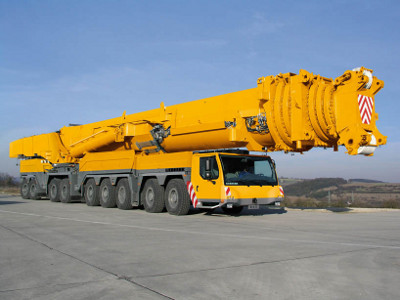
\includegraphics[width=.7\textwidth]{img/ltm11200.jpg}
\caption{Guindaste hidráulico da Liebherr - Modelo LTM-112OO 9.1}
\end{figure}

Como o equipamento possui rodas ele é transportado em rodovias comuns, porém, para ser operado, é necessário que ele seja montado sobre suas patolas, que o mantém estabilizado durante a operação. Essas patolas são retráteis e são sempre apoiadas sobre vigas de madeira ou chapas de metal, para aumentar a área e diminuir a pressão exercida no solo. O processo de patolamento de um guindaste precede qualquer operação e é essencial para a segurança da operação. São utilizados sempre níveis, sejam eles analógicos ou digitais, para garantir que o equipamento está alinhado com a horizontal, garantindo assim que suas forças sejam igualmente distribuídas pelas 4 patolas (alguns equipamentos possuem uma quinta patola embaixo da cabine do motorista).

\begin{figure}[H]
\centering
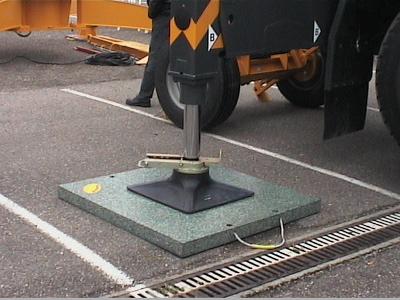
\includegraphics[width=.6\textwidth]{img/patolamento.jpg}
\caption{Detalhe de um guindaste patolado}
\end{figure}

Muitos dos equipamentos ainda em uso no Brasil possuem pelo menos uma década, o que faz com que o parque de guindastes do país possua todo o tipo de tecnologia para nivelamento. Os mais antigo possuem apenas um nível bolha redondo enquanto os mais recentes já vem com sistemas eletrônicos embutidos. No meio do caminho entre esses dois existem vários equipamentos que tiveram seus sistemas atualizados e ganharam sensores de inclinação mais modernos.

Observando esse cenário comecei a ver a variedade de fabricantes dos inclinômetros, percebendo inclusive que alguns eram nacionais. Em conversa com meus superiores (trabalhando há mais de 10 anos com manutenção de guindastes), fui informado de que vários desses sistemas falhavam com frequência e que custavam, invariavelmente, mais de 2 mil reais. Com essa realidade em mente tive a idéia de desenvolver uma alternativa barata para esse tipo de função.

\begin{figure}[H]
\centering
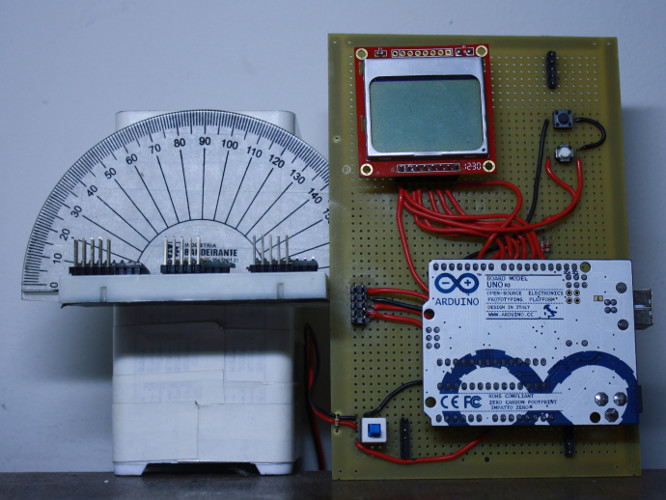
\includegraphics[width=.5\textwidth]{img/prototipo.jpg}
\caption{Protótipo finalizado}
\end{figure}


Ao pesquisar mais sobre microcontroladores logo me deparei com o Arduino, plataforma aberta de prototipagem que agilizou em muito o processo de prototipagem. Falaremos mais sobre ele no seção \ref{arduino}.Tivemos também de escolher o sensor mais adequado para o inclinômetro e acabamos usando uma combinação de dois deles, um acelerômetro e um giroscópio. Falaremos mais sobre eles na seção \ref{sensores}. Por fim, na seção \ref{filtros}, descrevemos a necessidade que tivemos de utilizar filtros algorítmicos para unir os valores dos dois sensores e diminuir os ruídos no resultado final.

O desenvolvimento desse projeto foi realizado de forma bastante experimental, sendo as pesquisas realizadas na vasta documentação disponível na internet e as peças compradas da China, por serem de baixíssimo custo e relativa qualidade. 

\begin{figure}[H]
\centering
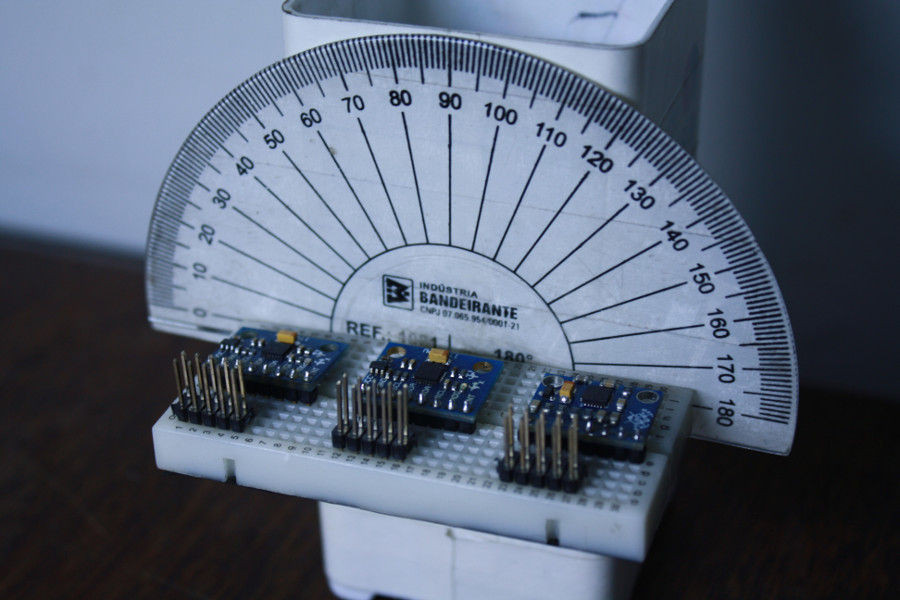
\includegraphics[width=.5\textwidth]{img/sensores.jpg}
\caption{Sensores em redundância utilizados nos testes}
\end{figure}


\subsection{Estado da Arte}

Fizemos uma pesquisa na internet com o intuito de descobrir quais as características mais comuns nos inclinômetros comerciais utilizados no Brasil. Vimos que diversas empresas, no Brasil e no mundo, fabricam esse tipo de equipamento para guindastes e guindautos. Um fator em comum entre todas elas é o fato de utilizarem de plataformas e softwares proprietários em seus equipamentos. Normalmente a precisão e o grau de proteção dos equipamentos são bem parecidos entre os fabricantes, as principais diferenças observadas foram os itens adicionais, como alarmes visuais e sonoros e visores adicionais, e os sensores agregados, como os sensores de pressão de patola e os de comprimento e inclinação da lança telescópica.

Conversando com os profissionais da STG, fiquei sabendo que em geral esses equipamentos são vendidos em pacotes de sensores, para serem utilizados em guindastes mais antigos que não possuem nenhum sensor de segurança.

Segue abaixo a lista das principais empresas do ramo localizadas na internet.

\begin{enumerate}
\item ComLink

\begin{itemize}
\item \textbf{Site:} \site{www.comlink.ind.br}
\item \textbf{Sede:} Ribeirão Preto - SP
\end{itemize}

Os equipamentos da ComLink variam apenas em quantidade de eventos que podem ser registrados e no tipo de conexão do sensor com o visor, podendo ser a cabo ou sem fio. Os inclinômetros têm resolução de $0,1^\circ$, possuem dois eixos de medição e proteção IP 67, contra poeira e submersão. Não foi encontrada informação sobre a precisão dos equipamentos.

\item Geodigitus

\begin{itemize}
\item \textbf{Site:} \site{www.geodigitus.com.br}
\item \textbf{Sede:} Belo Horizonte - MG
\end{itemize}

Seus equipamentos possuem resolução de $0,1^\circ$ e precisão de $0,5^\circ$. Possui 2 eixos de medição e proteção IP 65, contra poeira e jatos d'água.

\item Hirschmann

\begin{itemize}
\item \textbf{Site:} \site{www.hirschmann.com}
\item \textbf{Sede:} Estados Unidos da América
\end{itemize}

A Hirschmann é lider mundial de mercado em sensores para equipamentos de carga. Vários sistemas de outras empresas utilizam sensores deles e montam apenas os receptores e visores. Alguns de seus sensores possuem resolução de até $0,01^\circ$, proteção IP 69K contra poeira e jatos de água em altas temperaturas e pressões. Os sensores possuem ainda a opção sem fio ou com fio.

\item Load Control

\begin{itemize}
\item \textbf{Site:} \site{www.loadcontrol.com.br}
\item \textbf{Sede:} Porto Alegre - RS
\end{itemize}

A Load Control não fornece detalhes sobre seus produtos.

\item LSI

\begin{itemize}
\item \textbf{Site:} \site{www.loadsystems.com}
\item \textbf{Sede:} Estados Unidos da América
\end{itemize}

Os sensores da LSI possuem resolução de $0,1^\circ$ e precisão típica de $0,3^\circ$. Seus sensores são sem fio, com dois eixos e possuem proteção IP 66, contra poeira e jatos de água em alta pressão.

\item Mestria

\begin{itemize}
\item \textbf{Site:} \site{www.mestria.com.br}
\item \textbf{Sede:} Belo Horizonte - MG
\end{itemize}

A Mestria não fornece informações técnicas sobre seus produtos.

\item Tecnnic

\begin{itemize}
\item \textbf{Site:} \site{www.tecnnic.com.br}
\item \textbf{Sede:} Criciúma - SC
\end{itemize}

A Tecnnic produz equipamentos com resolução de $0,1^\circ$ e proteção IP 66.

\end{enumerate}

\subsection{Arduino}
\label{arduino}

 O conceito de \textit{open-source hardware} (hardware de código aberto), utilizado pelo Arduino (\href{http://arduino.cc}{arduino.cc}), determina que todos os projetos e especificações sejam liberados para uso e modificação por qualquer usuário. Com isso, nos últimos anos, surgiram dezenas (se não centenas) de versões modificadas dos seus projetos, cada uma com sua característica e aplicação específica. Essa versatilidade do Arduino fez com que ele se tornasse, pouco depois de seu surgimento, em 2005, referência para amadores e artistas ingressando no mundo da eletrônica. Hoje em dia ele já se consolidou como uma plataforma sólida e em constante expansão e vem sendo usado cada vez mais dentro de escolas técnicas e de engenharia para aprendizado de programação e eletrônica.
 
\begin{figure}[H]
\centering
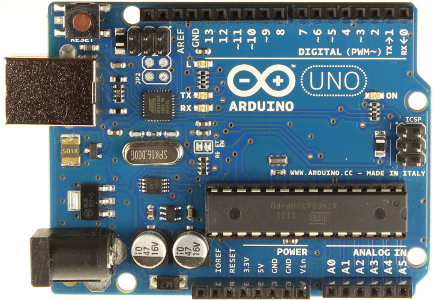
\includegraphics[width=.35\textwidth]{img/arduino1.jpg}
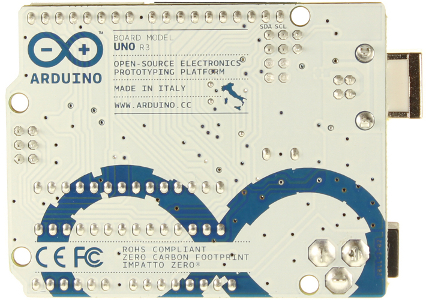
\includegraphics[width=.35\textwidth]{img/arduino2.jpg}
\caption{Arduino Uno R3 - Frente e verso}
\end{figure} 
 
O movimento \textit{open-source}, mais conhecido pelos softwares, foi importantíssimo para a evolução da tecnologia em várias áreas. Como exemplo temos o fato de os sistemas GNU/Linux, talvez o maior projeto de software livre do mundo, ter dominado o mercado de servidores, sistemas embutidos e, mais recentemente, de sistemas móveis, como celulares e tablets. Esse fato pouco lembrado sobre o software livre é essencial para se compreender a rápida evolução e a popularização desse tipo de tecnologia nas últimas décadas.
 
 O Arduino possui entradas e saídas digitais e analógicas que são programáveis por uma linguagem padrão baseada em Wiring, mas com a sintaxe semelhante a C/C++. Isso faz com que os códigos sejam facilmente modificados para projetos em plataformas semelhantes. Compramos para o projeto a versão \textit{Arduino Uno R3}, um dos modelos mais básicos. Suas especificações podem ser encontradas na tabela \ref{espec}.
 
 Os pinos digitais permitem que sejam lidos ou enviados sinais definidos pelo usuário em código. As entradas analógicas permitem a leitura de sensores de vários tipos, como de temperatura, de luz ou de movimento. Os limites de tensão da placa são bastante amplos, graças à fonte embutida na placa, que pode ser alimentada pelo conector, através de uma bateria ou fonte externa, ou então pela saída USB de qualquer computador. Os Arduinos já vem pré-programados com o que é chamado de \textit{bootloader}, um programa que inicializa o microcontrolador e o deixa pronto a ser reprogramado pelo computador através da porta USB.
 
\begin{table}[H]
\centering
\begin{tabular}{ll}
Microcontrolador	& ATmega328 \\
\hline
Tensão de Operação	& 5V \\
\hline
Tensão Recomendada	& 7-12V \\
\hline
Limites de tensão	& 6-20V \\
\hline
Pinos Digitais E/S	& 14 \\
\hline
Pinos Analógicos E	& 6 \\
\hline
Corrente por Pino& 40 mA \\
\hline
Corrente no pino 3.3V & 50 mA \\
\hline
Memória Flash		& 32 KB \\
\hline
Memória SRAM		& 2 KB \\
\hline
Memória EEPROM		& 1 KB\\
\hline
Velocidade de Clock	& 16 MHz\\
\end{tabular}
\caption{Especificações técnicas do Arduino Uno R3}
\label{espec}
\end{table}

Um dos grandes atrativos do Arduino é o preço acessível. A placa foi comprada por US\$ 15,20, o que, na época, equivalia a cerca de R\$ 35,00. Existem ainda cópias que podem chegar a U\$ 9,00 ou até menos. Como os projetos são abertos, é também possível montar seu próprio Arduino com peças compradas em qualquer loja de eletrônica.

Utilizando o Arduino Uno R3, uma placa de montagem rápida, um módulo com uma tela LCD monocromática, 2 botões e um sensor com um acelerômetro e um giroscópio montamos a primeira versão do protótipo. Essa tela foi originalmente projetada para o celular 5110, da Nokia, porém vem sendo muito utilizada por hobbystas por seu preço acessível e versatilidade de uso, sendo possível, inclusive, exibir gráficos com ela.

\begin{figure}[H]
\centering
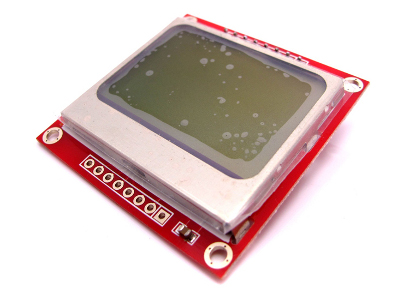
\includegraphics[width=.4\textwidth]{img/tela.jpg}
\caption{Módulo LCD para Arduino}
\end{figure}

\subsection{Sensores}
\label{sensores}

Sensores são dispositivos que reagem a um estímulo físico ou químico de maneira prevista e mensurável. Existem sensores para todos os tipos de aplicação: de medidores de gás carbônico a sensores elétricos dos mais variados. Cada um tem sua utilidade específica e mede grandezas diferentes. Da mesma forma, a interface de saída de um sensor pode variar dependendo da aplicação. Podemos ter sensores que variam a tensão de saída ou a corrente, ou ainda sensores digitais, que, por meio de sinais discretos e um protocolo estabelecido, realizam a transmissão dos dados de forma síncrona para a central.

Na execução desse protótipo, um grande problema foi a escolha dos sensores. Vi que a maior parte dos aparelhos que necessitam de medição de ângulo, utilizam uma combinação de acelerômetro e giroscópio. Estão incluídos ai a maior parte dos celulares de última geração e drones voadores, tanto amadores quanto profissionais. Existem inclusive placas que funcionam como piloto automático de drones voadores (com até 8 hélices) que são desenvolvidas baseadas em Arduino, como a APM, da 3DRobotics (\href{http://copter.ardupilot.com/wiki/common-apm25-and-26-overview/}{ardupilot.com}). Nesse caso a placa ainda vem com a opção de se utilizar um magnetometro, que funciona como uma búlsola, ao medir o campo magnético da terra.

\begin{figure}[H]
\centering
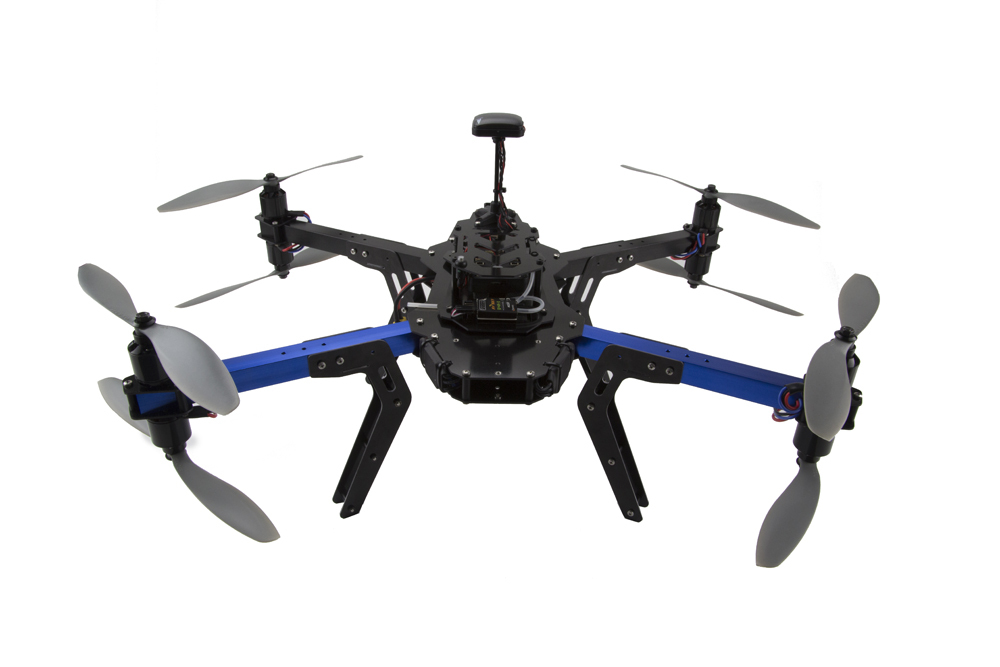
\includegraphics[width=.5\textwidth]{img/copter.jpg}
\caption{Quadricóptero comercial baseado em Arduino}
\end{figure}

Ao combinar mais de um sensor é possível otimizar a medição individual deles, pois todo sensor possui algum tipo de ruído que interfere em sua leitura. Optamos por utilizar o acelerômetro e o giroscópio, primeiramente por serem complementares, no sentido de que um possui um ruído de alta frequência enquanto o outro possui um de baixa frequência. Além disso é possível encontrar no mercado, com muita facilidade, modelos bastante baratos e seu uso é amplamente documentado na internet, incluindo várias bibliotecas já desenvolvidas para diversos fins.

\subsubsection{Acelerômetro}

Cada vez mais empregados em aparelhos eletrônicos dos mais variados, como celulares e tablets, os acelerômetros já são utilizados na industria, principalmente de aviação e espacial, há décadas. Porém foi com sua popularização na industria automobilística que a produção em massa desses sensores chegou ao ponto de torná-lo acessível para o grande público.

Como o próprio nome diz, um acelerômetro é um dispositivo que responde à variação da aceleração exercida sobre ele através de um sinal elétrico. No caso, como estamos todos sujeitos à aceleração da gravidade, um acelerômetro parado ao nível do mar sofre uma aceleraçào de $g=9,81 \frac{m}{s^2}$ enquanto em queda livre sua aceleração será igual a 0. Os acelerômetros, por possuírem mais de um eixo, podem medir a variação da aceleração entre seus extremos e assim calcular o ângulo em que se encontram. Essa relação se dá na forma de uma função senoidal, conforme pode ser observado na figura \ref{curva}.

\begin{figure}[H]
\centering
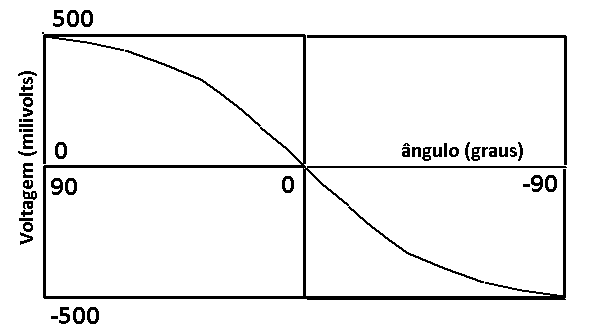
\includegraphics[width=.6\textwidth]{img/curva.png}
\caption{Relação típica entre o ângulo medido e a saída do acelerômetro}
\label{curva}
\end{figure}

Para entender melhor como funciona um acelerômetro podemos imaginar uma caixa em forma de cubo com uma bola no centro. Quando não houver aceleração alguma (em algum lugar no espaço sideral) a esfera flutuará no centro da caixa, sem tocar as faces internas (figura \ref{acel1}). Cada par de paredes opostas representa um eixo do sensor e a vista da figura não mostra a face $Y+$, que é o lugar do observador. Imaginemos então que cada parede é sensível à pressão e, quando aceleramos a caixa (a $1g = 9,8 \frac{m}{s^2}$) em uma direção a bola atingirá a face oposta, conforme mostrado na figura \ref{acel2}.

\begin{figure}[H]
\centering
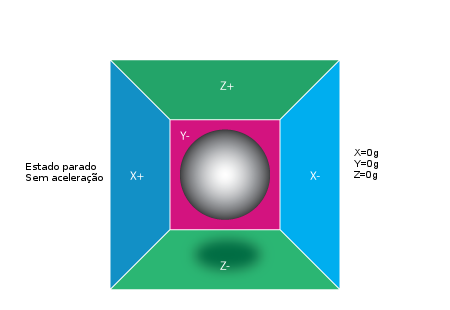
\includegraphics[width=.6\textwidth]{img/acel1.png}
\caption{Acelerômetro submetido a força $g=0$}
\label{acel1}
\end{figure}

É medida então a pressão exercida pela bola na parede $X-$, o que significa, na verdade, que a aceleração é no sentido oposto. Essa força é usualmente chamada de \emph{força inercial} ou \emph{força fictícia} e é representada pela seta vermelha na figura \ref{acel2}. Essa força no caso é causada por uma aceleração brusca, em um lugar onde não há força gravitacional atuando sobre o sistema. Porém, se levarmos nosso sensor para a Terra e posicionarmos no chão, estaremos o sujeitando à força da gravidade, que aqui é $g=9,8 \frac{m}{s^2}$, no nível do mar (figura \ref{acel3}).

\begin{figure}[H]
\centering
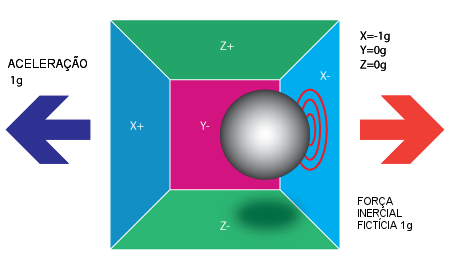
\includegraphics[width=.6\textwidth]{img/acel2.png}
\caption{Caixa com aceleração $1g=9,8 \frac{m}{s^2}$}
\label{acel2}
\end{figure}

Sobre o efeito da gravidade terrestre, a bola tocará a face $Z-$ da caixa, exercendo assim uma força sobre ela que será convertida em um sinal elétrico proporcional. O efeito seria igual ao de aproximar um imã dessa face caso a bola fosse de metal. É importante frisar que o acelerômetro mede diretamente a força, não a aceleração. As análises feitas até agora foram feitas considerando apenas 1 eixo do acelerômetro por vez. Isso não é exatamente útil no caso de análise de ângulos em 3 dimensões, que pode ser feito usando um acelerômetro de 3 eixos.

\begin{figure}[H]
\centering
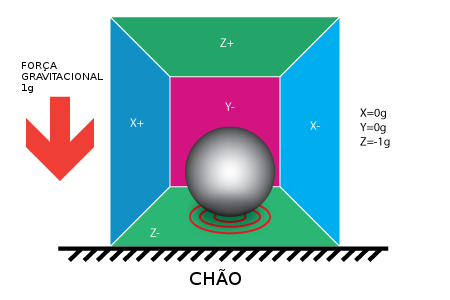
\includegraphics[width=.6\textwidth]{img/acel3.png}
\caption{Caixa sujeita à força da gravidade de $1g=9,8 \frac{m}{s^2}$}
\label{acel3}
\end{figure}

Ao posicionarmos o sensor em um ângulo entre os eixos, a esfera tocará mais de uma face simultâneamente. Com isso, a força exercida sobre cada uma será uma componente da força peso total, permitindo o cálculo do ângulo em relação à horizontal, conforme mostrado na figura \ref{acel4}. Dessa forma, o módulo das componentes nas paredes $Z-$ e $X-$ será de aproximadamente $0,71g$, caso o ângulo da caixa seja de $45^\circ$.

\begin{figure}[H]
\centering
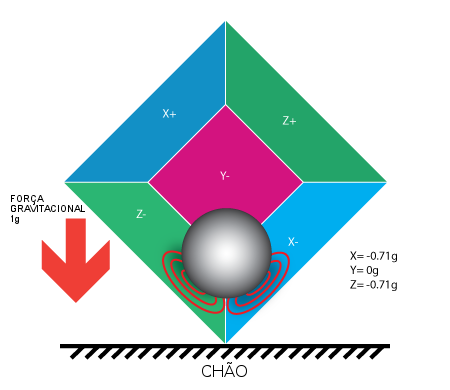
\includegraphics[width=.6\textwidth]{img/acel4.png}
\caption{Caixa inclinada sujeita à força da gravidade}
\label{acel4}
\end{figure}

Até agora apresentamos o modelo considerando que a força gravitacional estaria sempre para baixo, porém, para os cálculos, é mais interessante que o sistema de coordenadas do acelerômetro seja fixado como referência e a força aplicada sobre ele gire em torno de sua origem. Podemos observar essa configuração na figura \ref{eixos1}, onde $X$, $Y$ e $Z$ são as bases do sistema, $R$ é a força aplicada sobre o acelerômetro e $R_x$, $R_y$ e $R_z$ são as componentes de $R$ no sistema de coordenadas.

\begin{figure}[H]
\centering
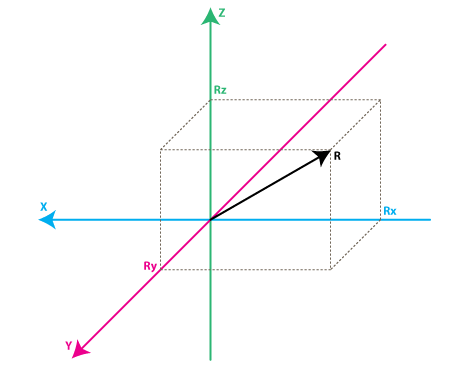
\includegraphics[width=.5\textwidth]{img/eixos1.png}
\caption{Sistema de coordenadas utilizado no modelo do acelerômetro}
\label{eixos1}
\end{figure}

Nesse modelo, temos os eixos perpendiculares às faces da caixa do outro modelo. Dessa forma, é simples calcular o vetor $R$, utilizando o teorema de Pitágoras para 3 dimensões: $$R^2=R_x^2+R_y^2+R_z^2$$ ou 

\begin{equation}
R=\sqrt{R_x^2+R_y^2+R_z^2}
\label{pit3d}
\end{equation}

\medskip
Como já dissemos, acelerômetros podem ser classificados entre digitais e analógicos. Os analógicos fornecem uma tensão em um faixa pré-definida e esse valor deve ser convertido em digital utilizando um conversor analógico para digital, assunto já fora do escopo desse trabalho. Por sua vez, os sensores digitais fornecem a informação por meio de um protocolo, como SPI, USART ou I$^2$C. Independente do formato em que o sensor entrega os dados ele será convertido em um valor digital em uma determinada faixa, dependendo da precisão do sensor. Por exemplo, um microprocessador com 10 bits de precisão lerá valores entre 0 e 1023,  pois $2^{10}-1=1023$.


\begin{figure}[H]
\centering
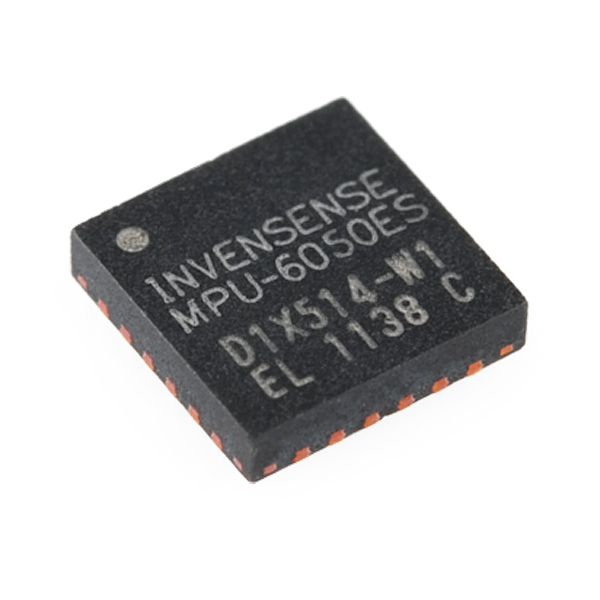
\includegraphics[width=.4\textwidth]{img/chip2.jpg}
\caption{MPU 6050 - Giroscópio e acelerômetros integrados num chip digital}
\end{figure}


Optamos por utilizar um chip digital pela facilidade da manipulação dos dados. Ecolhemos o modelo MPU 6050, fabricado pela InvenSense (\href{http://www.invensense.com/}{invensense.com}), que possui um acelerômetro e um giroscópio, cada um com 3 eixos. Além disso, ele pode ser integrado a um compasso de até 3 eixos ou ainda a outros sensores, graças a seus protocolos digitais, SPI e I$^2$C.

Esse mesmo chip é utilizado em diversos aparelhos celulares comerciais, para implementar interfaces de movimento nos equipamentos. Por suas proporções reduzidas e por utilizar soldagem SMD, optamos por comprar um módulo para Arduino com esse chip, uma vez que ele já vem com a interface necessário para conversar com o microcontrolador. Escolhemos um modelo que custou US\$ 11,40, o equivalente a cerca de R\$ 25,00, semelhante ao da figura \ref{chip1}.


\begin{figure}[H]
\centering
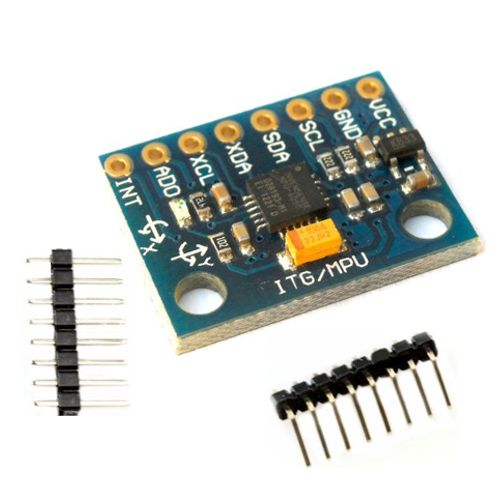
\includegraphics[width=.4\textwidth]{img/chip.jpg}
\caption{Módulo para Arduino utilizando o MPU 6050}
\label{chip1}
\end{figure}

Suponhamos então que, em certa medição, lemos os seguintes resultados do acelerômetro, já convertidos pelo conversor analógico digital 

$$AcR_x=520$$ 
$$AcR_y=667$$ 
$$AcR_z=589$$

Cada conversor desse tipo possui uma tensão de referência, no nosso caso 3,3V, que será utilizada para converter o valor digital em uma tensão, através de uma simples regra de três: 

$$\left\{\begin{array}{rcl}
V_{R_{x}} &\longrightarrow & V_{ref}\\
AcR_x &\longrightarrow & P_{Ac}
\end{array}\right.
$$
onde 

\begin{center}
\begin{tabular}{rcl}
$V_{R_x}$ & $\longrightarrow$ & tensão lida do sensor \\
$V_{ref}$ & $\longrightarrow$ & tensão de referência utilizada \\
$AcR_x$ & $\longrightarrow$ & valor digital lido do sensor \\
$P_{Ac}$ & $\longrightarrow$ & valor digital máximo alcançado pelo sensor
\end{tabular}
\end{center}
no nosso caso teríamos 

$$V_{R_x} = \frac{AcR_x\ast3,3}{1023}$$ 

Analogamente, para cada uma das leituras do acelerômetro, teríamos

$$V_{R_x} = \frac{520\ast3,3}{1023} \simeq 1,68 V$$

$$V_{R_y} = \frac{667\ast3,3}{1023} \simeq 2,15 V$$

$$V_{R_z} = \frac{589\ast3,3}{1023} = 1,90 V$$

que seria a leitura, em volts, do valor enviado pelo sensor para cada um dos eixos.

Todo acelerômetro possui um valor de tensão para zero-g ($V_{zero-g}$), em torno do qual o sensor variará seu sinal de saída. Esse valor pode ser encontrado no manual do sensor e, para o nosso caso, é de $1,65V$. Podemos calcular a variação de voltagem em torno do valor de zero-g conforme mostrado abaixo:

$$\Delta V_{R_x} = 1,68V - 1,65V=0,03V$$

$$\Delta V_{R_y} = 2,15V - 1,65V=0,50V$$

$$\Delta V_{R_z} = 1,90V - 1,65V=0,25V$$

Temos nossa leitura dos valores em volts, porém precisamos agora de conseguí-las em $g\ (9,8m/s^2)$, ou seja, em valores de aceleração. Para tal, precisamos encontrar o valor de sensibilidade, este também contido nas especificações do sensor, que é normalmente representado em $mV/g$. Com a sensibilidade de $478,5mV/g = 0,4785 V/g$ podemos aplicar esse valor na fórmula da seguinte maneira:

$$R_x = \frac{\Delta V_{R_x}}{Sensibilidade}$$

\medskip
\noindent
o que aplicado aos nossos valores nos daria

$$R_x=\frac{0,03 V}{0,4785 V/g}\simeq0,06g$$

$$R_y=\frac{0,50 V}{0,4785 V/g}\simeq1,04g$$

$$R_z=\frac{0,25 V}{0,4785 V/g}\simeq0,52g$$

Naturalmente, poderíamos juntar todos os passos em apenas uma fórmula, como fazemos de fato no código do programa. A descrição passo a passo das contas foi feita apenas para fins didáticos. Teríamos então:

\begin{equation}
R_x=(\frac{AcR_x\ast V_{ref}}{1023}-V_{zero-g})/Sensibilidade
\label{eq2}
\end{equation}

$$R_y=(\frac{AcR_y\ast V_{ref}}{1023}-V_{zero-g})/Sensibilidade$$

$$R_z=(\frac{AcR_z\ast V_{ref}}{1023}-V_{zero-g})/Sensibilidade$$

Temos agora os valores das componentes de $R$, com os quais é possível calcular não só $R$ como os ângulos entre $R$ e as origens do sistema. É possível calcular o ângulo entre 1 ou mais origens, de forma a termos uma noção completa de qual a inclinação do sensor no espaço. O cálculo dos ângulos envolve alguma trigonometria, porém nada que fuja do habitual. Na figura \ref{eixos2} definimos os ângulos entre $R$ e os eixos de coordenadas como $A_{xr}$, $A_{yr}$ e $A_{zr}$.

\begin{figure}[H]
\centering
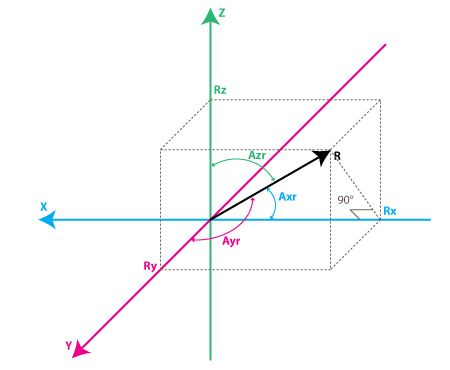
\includegraphics[width=.5\textwidth]{img/eixos2.png}
\caption{Eixos do sistema de coordenadas com os ângulos indicados}
\label{eixos2}
\end{figure}

Da figura \ref{eixos2} podemos deduzir que o cosseno de qualquer um desses ângulos pode ser calculado pela sua componente no eixo correspondente sobre $R$. Como pela equação \ref{pit3d} conseguimos calcular o valor de $R$, podemos fazer então calcular o ângulo através da função inversa do cosseno, o arco-cosseno.

$$\cos(A_{xr})=\frac{R_x}{R}$$

$$\cos(A_{yr})=\frac{R_y}{R}$$

$$\cos(A_{zr})=\frac{R_z}{R}$$

\noindent\medskip
usando a função inversa temos

$$A_{xr}=\arccos(\frac{R_x}{R})$$

$$A_{yr}=\arccos(\frac{R_y}{R})$$

$$A_{zr}=\arccos(\frac{R_z}{R})$$

Finalmente temos o valor medido pelo acelerômetro. Com esses dados em mãos é possível analisar a posição do sensor e dizer se ele está nivelado ou não. Temos um problema com o acelerômetro que é seu ruído de alta frequência, como ele mede diretamente a variação da força exercida sobre ele e é muito sensível, mesmo com o equipamento parado sobre uma mesa há uma variação dos valores lidos. Como independente do tempo de espera essa variação não aumenta ou diminui, esse ruído é chamado de alta frequência. O giroscópio, apresentado em seguida, possui características diferentes, o que faz com que ele em um curto espaço de tempo seja bastante confiável, enquanto ao longo do tempo seu erro aumente. Esse tipo de ruído é chamado de baixa frequência, pois acontece ao longo do tempo.

\subsubsection{Giroscópio}

De forma totalmente distinta do acelerômetro, o giroscópio não é bem representado pelo modelo da caixa com a bola flutuando. Esse sensor é originalmente constituído por um disco girando sobre uma estrutura de até 3 anéis, cada um com giro livre em um eixo (figura \ref{giro}). Quando o disco se pôe a girar ele gera uma força resultante que se opõe a qualquer tentativa de giro que seja feita no sensor. Ele ainda pode ser movido paralelamente ao seus eixos sem interferir na medição, porém qualquer mínima alteração no giro será percebida.

\begin{figure}[H]
\centering
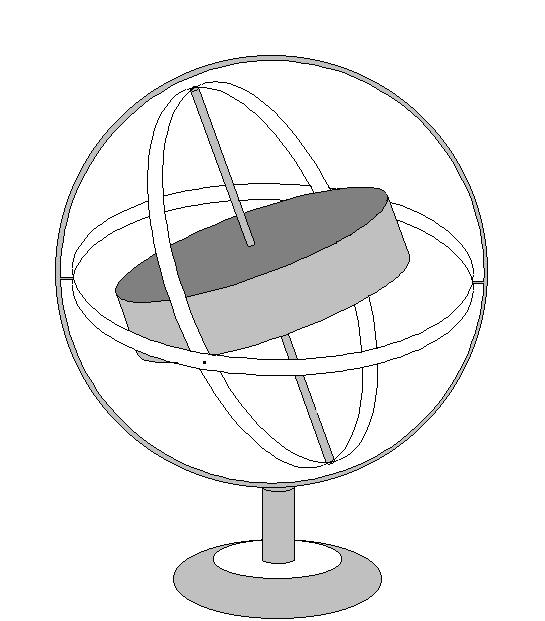
\includegraphics[width=.4\textwidth]{img/giro.jpg}
\caption{Modelo de giroscópio mecânico}
\label{giro}
\end{figure}

Uma combinação de 2 giroscópios é comunmente usada em aviões e naves espaciais para navegação. São usados porém giroscópios mecânicos agregados a sensores elétricos ou ópticos, para aumentar a precisão do sensor. O modelo de giroscópio eletrônico que usamos não possui partes mecânicas e, por isso, é menos preciso. Apesar disso ele é bastante útil para aplicações não tão críticas quanto navegação espacial!

\begin{figure}[H]
\centering
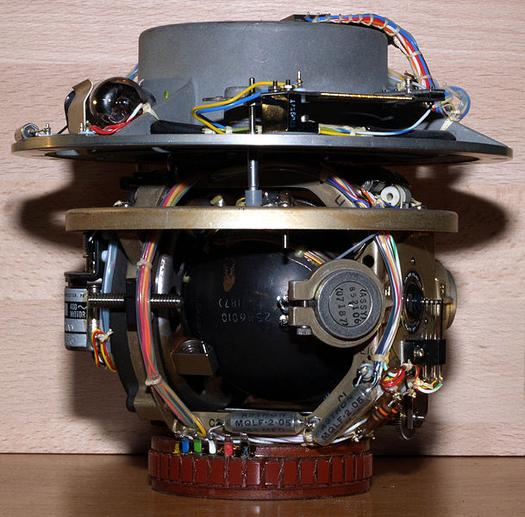
\includegraphics[width=.5\textwidth]{img/giro2.jpg}
\caption{Giroscópio óptico para navegação}
\label{giro2}
\end{figure}

Para entendermos como é calculado o ângulo utilizando o giroscópio, é importante analisarmos o sistema de coordenadas da figura \ref{eixos3}, utilizado no modelo.

\begin{figure}[H]
\centering
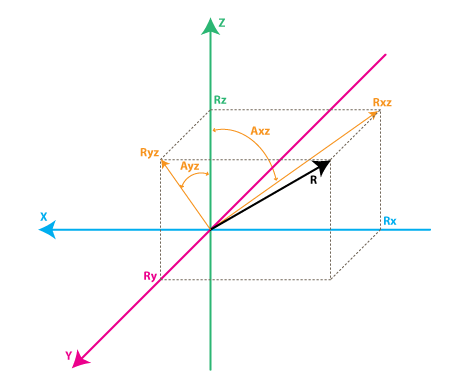
\includegraphics[width=.5\textwidth]{img/eixos3.png}
\caption{Sistema de coordenadas utilizado no modelo do giroscópio}
\label{eixos3}
\end{figure}

 Definamos primeiramente 

$$R_{xz} \longrightarrow \mbox{projeção de }R\mbox{ no plano }XZ$$

$$R_{yz} \longrightarrow \mbox{projeção de }R\mbox{ no plano }YZ$$

Considerando o triângulo retângulo formado por $R_{xz}$ e $R_z$ e utilizando o teorema de Pitágoras temos:

$$R_{xz}^2=R_x^2+R_z^2$$ e de forma semelhante

$$R_{yz}^2=R_y^2+R_z^2$$

Esses valores servem apenas de demonstração das relações entre os vetores analisados, o que nos interessa, entretanto, são os ângulos $A_{xz}$ e $A_{yz}$, que podem ser definidos como:

$$A_{xz} \longrightarrow \mbox{ângulo entre }R_{xz}\mbox{ e o eixo }Z$$

$$A_{yz} \longrightarrow \mbox{ângulo entre }R_{yz}\mbox{ e o eixo }Z$$

O giroscópio mede, na realidade, a taxa de variação desses ângulo, que representam o giro em torno do eixo $Y$ e $X$, respectivamente. Para entendermos o que é a taxa de variação, nesse caso, podemos exemplificar da seguinte forma: imagine que medimos o ângulo $A_{xz}$ no momento $t_0$, chamaremos esse valor de $A_{xz_0}$. Da mesma forma mediremos esse ângulo no momento $t_1$, nomeando-o de $A_{xz_1}$. A taxa de variação do ângulo seria calculada da seguinte forma:

$$\Delta A_{xz}=\frac{A_{xz_1}-A_{xz_0}}{t_1-t_0}$$ ou ainda

$$\Delta A_{xz}=\frac{A_{xz_1}-A_{xz_0}}{\Delta t}$$

Caso representemos o ângulo em graus e o tempo em segundos teremos, ao fim, um valor em $^\circ/s$. Esse é o valor lido pelo giroscópio. Assim como com o acelerômetro, o giroscópio não fornece uma saída diretamente proporcional a grandeza que queremos, logo teremos de calcular a taxa de variação do ângulo usando uma fórmula similar à equação \ref{eq2}, a qual nos referimos anteriormente.

$$\Delta A_{xz}=(\frac{Giro_{xz}\ast V_{ref}}{P_{gi}}-V_{\Delta zero})/Sensibilidade$$ e, de forma semelhante

$$\Delta A_{yz}=(\frac{Giro_{yz}\ast V_{ref}}{P_{gi}}-V_{\Delta zero})/Sensibilidade$$

\noindent\medskip
onde

\begin{center}
\begin{tabular}{rcl}
$\Delta A_{xz}$ e $\Delta A_{yz}$ & $\longrightarrow$ & a taxa de variação angular em $^\circ/s$ \\
$Giro_{xz}$ e $Giro_{yz}$ & $\longrightarrow$ & o valor digital lido do giroscópio \\
$V_{ref}$ & $\longrightarrow$ & valor de tensão de referência \\
$Sensibilidade$ & $\longrightarrow$ & sensibilidade fornecida pelo fabricante em $\frac{mV}{^\circ/s}$\\
$P_{gi}$ &$\longrightarrow$& precisão do microcontrolador \\
$V_{\Delta zero}$&$\longrightarrow$& valor de tensão para giro zero, fornecido pelo fabricante
\end{tabular}
\end{center}

Tomemos como exeplo os seguintes valores lidos pelo Arduino do giroscópio:

$$Giro_{xz}=580$$

$$Giro_{yz}=297$$

Com as fórmulas e as especificações do giroscópio podemos calcular a taxa de variação angular:

$$\Delta A_{xz}=(\frac{580\ast 3,3V}{1023}-1,23)/0,002\frac{V}{^\circ/s}\simeq 320^\circ/s$$

$$\Delta A_{yz}=(\frac{297\ast 3,3V}{1023}-1,23)/0,002\frac{V}{^\circ/s}\simeq -136^\circ/s$$

Podemos ver que o sensor gira em torno do eixo $Y$ (ou no plano $XZ$) com uma velocidade de $320^\circ/s$ e em torno do eixo $X$ (ou no plano $YZ$) com uma velocidade de $-136^\circ/s$. Esse valor ainda não representa o ângulo, mas é uma taxa de variação dele. Dessa forma podemos integrar o valor para chegar no ângulo do sensor. A fórmula para isso seria:

$$A_{xz} = \int_{t_0}^{t_ 1}\Delta A_{xz}dt$$

\noindent\medskip
sendo $t_0$ e $t_1$ os tempos de início e fim da medição. A explicação dessas ferramentas matemáticas foge ao escopo desse relatório, porém é interessante compreender que uma integral é uma soma infinitesimal de uma função, ou seja, ao se integrar, consegue-se a área debaixo da curva. Essa área, no caso do gráfico de $^\circ/s\times s$, representa o ângulo pois $$\frac{graus}{segundo}* segundo=grau$$

O giroscópio, por suas características, mantém uma precisão muito boa em curtos períodos de tempo, principalmente quando em movimento, porém, ao longo do tempo, ocorre o que é chamado de \emph{arrasto}. Esse efeito faz com que a medida lida pelo sensor varie irreversivelmente com o passar do tempo, gerando um ruído de baixa frequência. Porém, em conjunto com outros sensores, é possível utilizar as características positivas para se aumentar a precisão da medida.

Existem várias formas de se unir os valores dos sensores em um só. Na seção \ref{filtros} falaremos mais sobre o filtro complementar e o filtro de Kalman, as duas alternativas testadas em nossos experimentos, além da leitura individual dos sensores.

\subsection{Filtros}
\label{filtros}

Filtros são utilizados em todas as áreas técnicas para retirar partes indesejadas. Na hidráulica retira partículas dos líquidos, na eletrônica retira frequências específicas do sinal elétrico e, quando usado em um algoritmo, pode servir por, exemplo, para remover o ruído criado pelos sensores de inclinação. Cada sensor possui um tipo de ruído diferente, no caso do acelerômetro temos um ruído de alta frequência, enquando no giroscópio o ruído é de baixa frequência.

Nos experimentos que fizemos com nosso protótipo realizamos a leitura e o cálculo do ângulo usando os sensores individualmente e combinados utilizando dois filtros diferentes, o filtro complementar e o de Kalman. Falaremos mais sobre eles separadamente a seguir.

\subsubsection{Filtro Complementar}

O filtro complementar é uma aplicação particular do filtro de Kalman, discutido mais à frente. Como não há uma descrição estatística do ruído do problema, como no filtro de Kalman, a matemática se torna bem mais simples. Fazemos, basicamente, uma média ponderada dos dois valores, sendo cada peso a ``confiança" atribuída aquela medida. Um filtro complementar pode ser representado conforme a figura \ref{complementar}, sendo $x$ e $y$ leituras com ruídos de algum sinal $z$ e $\hat{z}$ o valor estimado pelo filtro complementar para $z$.

\begin{figure}[H]
\centering
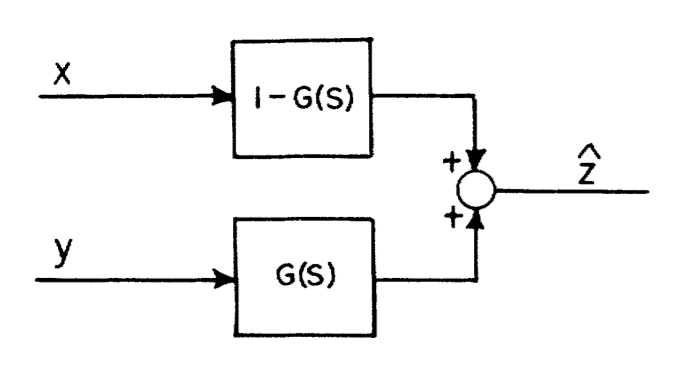
\includegraphics[width=.7\textwidth]{img/complementar.png}
\caption{Modelo de filtro complementar}
\label{complementar}
\end{figure}

Suponhamos que o ruído em $x$ seja de baixa frequência, como o do giroscópio, e o de $y$ seja de alta frequência, como o do acelerômetro. Teríamos de fazer então de $G(s)$ um filtro passa baixa para filtrar o ruído de alta frequência de $y$. $[1-G(s)]$ seria então o complemento de $G(s)$, logo, um filtro passa alta. Nesse tipo de filtro não são consideradas mais características do ruído.

Podemos tirar desse modelo a seguinte fórmula, utilizada em nosso código para cálculo da inclinação: 

\begin{equation}
\hat{z}=G(s)*x+[1-G(s)]*y
\end{equation}

Os valores de $G(s)$ e $[1-G(s)]$ foram primeiramente estimados e então otimizados durantes os testes.
\subsubsection{Filtro de Kalman}

O filtro de Kalman é um algoritmo recursivo que foi inventado por Rudolf E. Kálmán ($\star$ 19/5/1930 - ), húngaro erradico nos Estados Unidos. Desde sua criação, em torno de 1960, ele vem sendo utilizado em diversas aplicações, como processamento de sinais, controle de sistemas, navegação e etc. Inicialmente ele foi projetado para auxiliar na previsão da trajetória do projeto Apolo, da NASA. O algorítmo foi então incorporado ao computador da nave e, desde então, já foi utilizado diversas vezes pelo governo dos EUA, dos mísseis Tomahawk à torpedos e mísseis cruzadores aéreos.

Esse algoritmo envolve uma análise estatística do ruído apresentado, além de diversas manipulações com matrizes, sendo necessária a aplicação várias técnicas que fogem ao escopo desse trabalho. Pesquisando e conversando melhor com profissionais que utilizam o filtro de Kalman no dia-a-dia, descobrimos que normalmente o ajuste das variáveis é feito com testes exaustivos de várias combinações diferentes dos valores das variáveis.

Como o objetivo do trabalho não envolvia a implementação do filtro de Kalman, optamos por utilizar uma biblioteca para Arduino com o filtro já implementado. O código utilizado foi desenvolvido por Kristian Lauszus, do site \href{http://www.tkjelectronics.dk/}{TKJelectronics.dk}. Essa implementação foi testada por diversos internautas e é bastante simples, além de ser detalhadamente explicada no blog de seu site. O filtro de Kalman é vastamente documentado, tanto em livros quanto na internet, por sua vasta utilização em diversas áreas.

Veremos agora alguns trechos importantes do código, enquanto a implementação completa será reservada para os anexos, no capítulo \ref{anexos}.

\subsection{O Código}

Todo microcontrolador funciona em um \textit{loop} de execução no qual se verificam as leituras dos sensores, executam-se os cálculos e tarefas necessárias (como escrever ou ler da memória) e, finalmente, escreve-se nas saídas, sejam elas motores, luzes ou acionadores de qualquer tipo. Naturalmente essa ordem pode ser alterada, dependendo da aplicação do código, porém é importante compreender que o funcionamento desse tipo de aparelho ocorre dessa forma.

Vejamos então o loop principal do nosso código:

\newpage
{\singlespace\begin{lstlisting}
void loop() {
  
  // Sub-rotina de calibragem
  calibra();
  
  // Luz do visor
  ligaLuz();

  // Escreve no visor
  escreveDados(1);
  
  // Atualiza valores  
  atualizaValores();
  
  // Atualiza contador
  timer = micros();  
}
\end{lstlisting}
}

Podemos observar na linha 4 a função calibra() , que será detalhada mais à frente, que inicia o processo de calibragem, caso o botão calibrar seja apertado por mais de 5 segundos. Em seguida verificamos se o botão da luz traseira da tela foi pressionado com a função ligaLuz(), na linha 7. A função escreveDados() exibe os dados lidos e calculados no visor. O parâmetro recebido por ela, na linha 10 do código acima, foi adicionado para depuração. Ao se passar 1 para a função ele exibe os valores também no terminal serial, quando o valor é zero ele exibe os valores apenas na tela. A função atualizaValores(), na linha 13 realiza a leitura dos sensores e os cálculos de ângulo enquanto na linha 16 temos apenas a leitura do tempo atual, necessário para a integração dos valores do giroscópio.

Além da função de \textit{loop}, os microcontroladores possuem também, comunmente, uma função de \textit{setup}, que é executada apenas uma vez, ao se ligar o equipamento. Na função \textit{loop} que utilizamos foram mantidos trechos do exemplo original, retirado do site TKJelectronics.dk, e mantidos os comentários do autor.

{\singlespace\begin{lstlisting}
void setup() {  
  
  //Inicializa comunicacao serial com o computador
  Serial.begin(115200);
  
  //Inicializa o visor LCD
  myGLCD.InitLCD();
  myGLCD.setFont(SmallFont);
  
  myGLCD.print("Iniciando...", LEFT, 0);
  
  Wire.begin();
  
  i2cData[0] = 7; // Set the sample rate
  i2cData[1] = 0x00; // Configure gyro and acc filtering
  i2cData[2] = 0x00; // Set Gyro Full Scale Range
  i2cData[3] = 0x00; // Set Accelerometer Full Scale Range
  while(i2cWrite(0x19,i2cData,4,false)); // Write all registers
  while(i2cWrite(0x6B,0x01,true)); // Disable sleep mode
  
  while(i2cRead(0x75,i2cData,1));
  if(i2cData[0] != 0x68) { // Read "WHO_AM_I" register
    myGLCD.print("ERRO NO SENSOR!", LEFT, 8);
    //Serial.print(F("Error reading sensor"));
    while(1);  
  }
  
  delay(100); // Wait for sensor to stabilize
  
  myGLCD.print("Sen. config.", LEFT, 8);
  
  /* Set kalman and gyro starting angle */
  while(i2cRead(0x3B,i2cData,6));
  accX = ((i2cData[0] << 8) | i2cData[1]);
  accY = ((i2cData[2] << 8) | i2cData[3]);
  accZ = ((i2cData[4] << 8) | i2cData[5]);
  // atan2 outputs the value of -Pi to Pi (radians)
  // see http://en.wikipedia.org/wiki/Atan2
  // We then convert it to 0 to 2Pi and then from radians to degrees
  accYangle = atan2(accX,accZ)*RAD_TO_DEG;
  accXangle = atan2(accY,accZ)*RAD_TO_DEG;
  
  kalmanX.setAngle(0); // Set starting angle
  kalmanY.setAngle(0);
  gyroXangle = accXangle;
  gyroYangle = accYangle;
  compAngleX = accXangle;
  compAngleY = accYangle;
        
  myGLCD.print("Sen. calibr.", LEFT, 16);  

  // Calibragem dos fatores do filtro de Kalman
  
  kalmanX.setQangle(0.01);
  kalmanX.setQbias(0.0003);
  kalmanX.setRmeasure(0.15);

  kalmanY.setQangle(0.01);
  kalmanY.setQbias(0.0003);
  kalmanY.setRmeasure(0.15);
  
  myGLCD.print("Filtro calibr.", LEFT, 24);

  // Calibragem do angulo inicial
  calibragem = EEPROM.readDouble(0);
  
  // Luz do visor
  pinMode(pinoBotaoLed, INPUT);
  pinMode(pinoLed, OUTPUT);
  
  digitalWrite(pinoLed, statusLed);
  
  // Botao de Calibragem
  
  pinMode(pinoCalibr, INPUT);
  
  myGLCD.print("PRONTO!", LEFT, 32);
  delay(3000);
  
  timer = micros();
}
\end{lstlisting}}

Entre as linhas 4 e 29 temos a inicialização da comunicação serial com o computador (caso o Arduino esteja ligado via USB no computador), da tela e dos sensores, já os configurando da forma desejada. Importante frisar que, na linha 28, temos uma pausa que é dada aguardando a inicialização do sensor, de forma evitar leituras equivocadas enquanto o sensor se configura. Entre as linhas 33 e 48 é feita a leitura inicial dos sensores (fazemos a leitura sempre em dois eixos, $X$ e $Y$). A calibragem dos parâmetros do filtro é feita entre as linhas 54 e 60. Temos então a leitura da última calibragem registrada, na linha 65 e, finalmente, da linha 68 a linha 80 temos a configuração dos pinos do Arduino e a leitura inicial do tempo. Podemos ver essa mensagem sendo exibida na figura \ref{inicia}.

\begin{figure}[H]
\centering
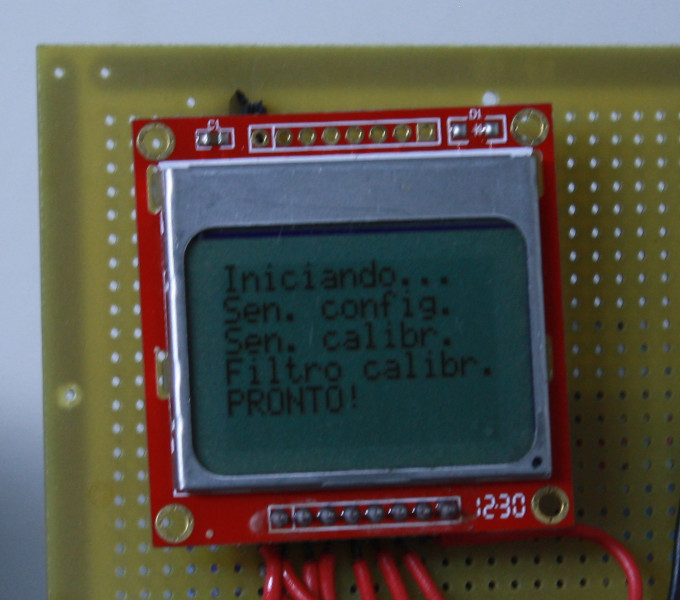
\includegraphics[width=.5\textwidth]{img/inicia.jpg}
\caption{Detalhe da inicialização do sistema}
\label{inicia}
\end{figure}

A função calibra() é necessária pois não sabemos em que posição o equipamento será instalado. É necessário, portanto, que o ângulo inicial seja calibrado usando uma ferramente externa de medição. No nosso caso usamos um transferidor fixado em uma base na qual o sensor girava. Dessa forma foi possível observar o ângulo do sensor de forma aproximada.

{\singlespace\begin{lstlisting}
void calibra(){

  leituraBotaoCalibr = digitalRead(pinoCalibr);

  // Botao pressionado, comeca a contagem
  if (leituraBotaoCalibr == HIGH && 
      ultimoStatusBotaoCalibr == LOW){
    tempoPressionado = millis();
  }
  
  // Botao pressionado por tempo maior que o configurado
  if (leituraBotaoCalibr == HIGH &&
      ultimoStatusBotaoCalibr == HIGH && 
      (millis()-tempoPressionado) > tempoAtivacao){
    myGLCD.clrScr();
    myGLCD.print("CALIBRAGEM", CENTER, 0);
    myGLCD.print("Nivele o ", LEFT, 16);
    myGLCD.print("equipamento.", LEFT, 24);
    myGLCD.print("Aperte o botao", LEFT, 32);
    myGLCD.print("uma vez.", LEFT, 40);

    delay(2000);

    leituraBotaoCalibr = digitalRead(pinoCalibr);

    while(leituraBotaoCalibr != HIGH){
      leituraBotaoCalibr = digitalRead(pinoCalibr);
      ultimoStatusBotaoCalibr = leituraBotaoCalibr;
      
      if(digitalRead(pinoBotaoLed) == HIGH){
        calibragem = 0;
        EEPROM.updateDouble(0,calibragem);
        myGLCD.clrScr();
        myGLCD.print("CALIBRAGEM 0", CENTER, 16);
        delay(3000);
        return;
      }
    }
    
    myGLCD.clrScr();
    myGLCD.print("CALIBRANDO", CENTER, 16);
    
    double valor = kalAngleX;
    
    for (int i = 0; i < 10; i++){
      
      atualizaValores();
      
      valor += kalAngleX;
      valor = valor/2;
      
      delay(200);
    }
    
    calibragem = valor;
    EEPROM.updateDouble(0,calibragem);

    myGLCD.clrScr();    
    myGLCD.print("PRONTO!", CENTER, 0);
    myGLCD.print("Equipamento", CENTER, 24);
    myGLCD.print("calibrado!", CENTER, 32);
    delay(3000);
  }
  
  ultimoStatusBotaoCalibr = leituraBotaoCalibr;

}
\end{lstlisting}}

Só entramos na função de calibragem caso tenhamos pressionado o botão para tal acima do tempo configurado no código (no caso 5 segundos). Essa rotina esta entre as linhas 3 e 14, onde entramos em uma condicional caso tenhamos pressioando o botão por esse tempo. Nesse ponto o usuário é então instruído a fazer nivelar o equipamento e pressionar o botão apenas uma vez. Nesse momento, se apertarmos o botão de acender o LED, teremos o que chamamos de ``calibragem 0", que é quando zeramos a variável de calibragem, considerando que o instrumento foi instalado no equipamento nivelado (linhas 30 a 37). Caso apertemos o botão de calibragem mais uma vez o Arduino faz uma média de 10 leituras do ângulo para servir como padrão (linhas 43 a 55). Finalmente o valor de calibragem é escrito na memória EEPROM, que não se apaga quando o Arduino é desligado e é lido novamente pelo programa na próxima religagem, de forma que, caso o aparelho continue imóvel nesse meio tempo não há necessidade de recalibragem.

\begin{figure}[H]
\centering
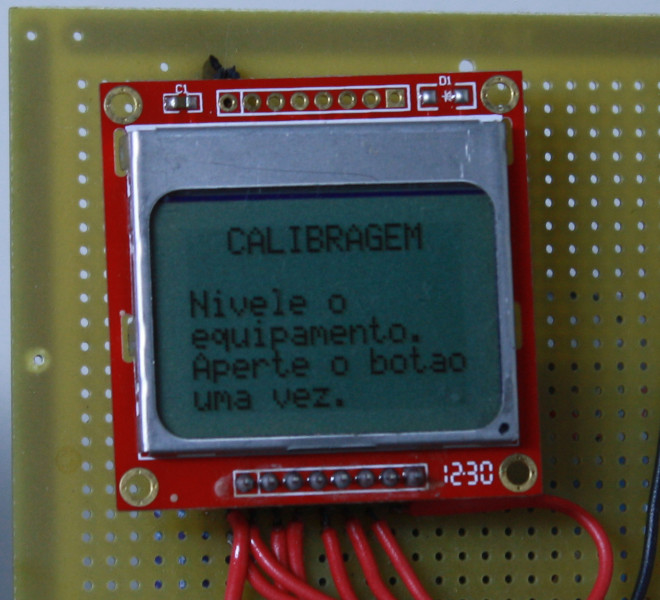
\includegraphics[width=.5\textwidth]{img/calibra.jpg}
\caption{Detalhe da calibração do sistema}
\label{calibra}
\end{figure}

Das funções essencias temos ainda a atualizaValores(), que faz de fato a leitura e os cálculos do ângulo.

{\singlespace\begin{lstlisting}
void atualizaValores(){
  while(i2cRead(0x3B,i2cData,14));
  accX = ((i2cData[0] << 8) | i2cData[1]);
  accY = ((i2cData[2] << 8) | i2cData[3]);
  accZ = ((i2cData[4] << 8) | i2cData[5]);
  gyroX = ((i2cData[8] << 8) | i2cData[9]);
  gyroY = ((i2cData[10] << 8) | i2cData[11]);
  gyroZ = ((i2cData[12] << 8) | i2cData[13]);
  
  accXangle = (atan2(accY,accZ))*RAD_TO_DEG;
  accYangle = (atan2(accX,accZ))*RAD_TO_DEG;
  
  //Calculo do angulo usando o giroscopio
  double gyroXrate = (double)gyroX/131.0;
  double gyroYrate = (double)gyroY/131.0;
  
  // Calculo sem filtros  
  gyroXangle += gyroXrate*((double)(micros()-timer)/1000000);
  gyroYangle += gyroYrate*((double)(micros()-timer)/1000000);
    
  //Calculo do angulo com filtro complementar
  compAngleX = (0.06*(compAngleX+
                (gyroXrate*(double)(micros()-timer)/1000000)))+
                (0.94*accXangle);
  compAngleY = (0.06*(compAngleY+
                (gyroYrate*(double)(micros()-timer)/1000000)))+
                (0.94*accYangle);
  
  //Calculo do angulo com filtro de Kalman
  kalAngleX = kalmanX.getAngle(accXangle, gyroXrate, 
               (double)(micros()-timer)/1000000);
  kalAngleY = kalmanY.getAngle(accYangle, gyroYrate, 
               (double)(micros()-timer)/1000000); 
}
\end{lstlisting}}

Como o sensor é digital, a leitura é feita por meio de um protocolo (linhas 2 a 9). Os ângulos \textit{accXangle} e \textit{accYangle} são calculados por meio da função atan2, que permite que se saiba em qual quadrante está o ângulo ao usar 2 parâmetros ao invés de apenas 1 (linhas 10 e 11). Fazemos então a conversão de radianos para graus, usando a constante da linguagem RAD\_TO\_DEG. Continuamos então os cálculos pelo giroscópio, dividindo seu valor pela precisão, de forma a termos a taxa de variação ângular (linhas 14 e 15). Em seguida temos o cálculo do ângulo feito integrando o valor lido pelo giroscópio (linhas 18 e 19), sem o uso de filtros. É importante observar que essa integração é feita iterativamente, de forma que ela é recalculada a cada passo. Pegamos então o valor lido pelo giroscópio em $^\circ/s$ e o multiplicamos pelo tempo atual menos o tempo lido na última iteração ($\Delta t$), dividido por 1 milhão, já que a função utilizada nos fornece o tempo em microsegundos.

\begin{figure}[H]
\centering
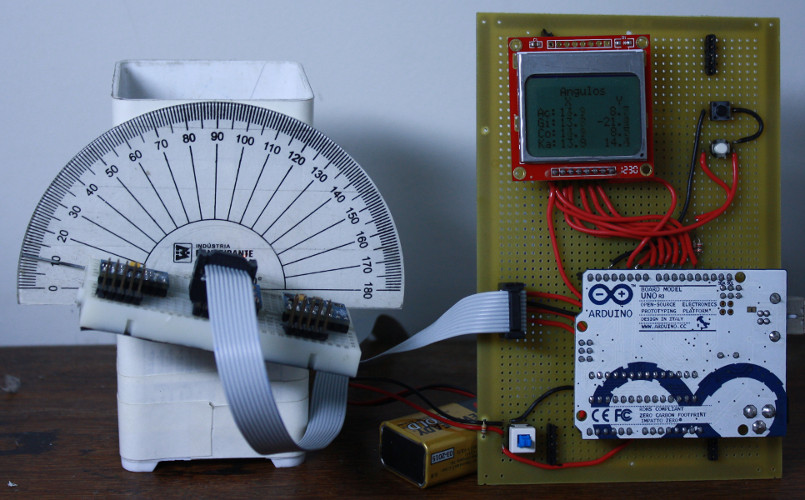
\includegraphics[width=.7\textwidth]{img/ligado.jpg}
\caption{Sistema ligado com o sensor angulado}
\label{ligado}
\end{figure}

Feito os cálculos sem filtro partimos para as medidas com filtro, começando pelo complementar. Utilizamos os fatores de $0,06$ para o giroscópio e $0,94$ para o acelerômetro (linhas 22 a 27), valores conseguidos empiricamente testando várias possibilidades e escolhendo esta como mais estável e precisa. Para calcularmos o ângulo usando o filtro de Kalman usamos uma biblioteca pronta, orientada a objetos, que nos fornece o ferramental ideal para tal tarefa. Após instanciadas as variáveis do filtro de Kalman ($kalAngleX$ e $kalAngleY$) podemos chamar a função getAngle(), que recebe como argumento o ângulo lido pelo acelerômetro, lido pelo giroscópio e a variação de tempo em segundos (linhas 30 a 33).

As demais funções e a biblioteca de filtro Kalman estão documentadas no capítulo \ref{anexos}, com seus códigos completos.

\section{Conclusão}

Para testarmos o  inclinômetro, fizemos com que na tela fossem exibidos os valores lidos para os eixos $X$ e $Y$ pelo acelerômetro e pelo giroscópio separadamente e os ângulos previstos pelo filtro complementar e de Kalman. Posicionamos o sensor em uma protoboard fixada em um eixo, de forma a podermos medir seu ângulo de inclinação por meio de um transferidor atrás da protoboard, conforme visto na figura \ref{detalhe}.

\begin{figure}[H]
\centering
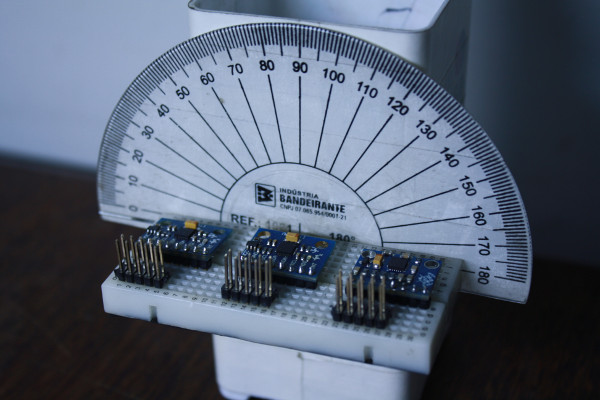
\includegraphics[width=.7\textwidth]{img/detalhe.jpg}
\caption{Módulo do protótipo com o inclinômetro}
\label{detalhe}
\end{figure}

Coletamos os dados medidos através da interface serial do Arduino e realizamos alguns testes afim de comparar as 4 diferentes formas de medição. No primeiro experimento iniciamos o sistema e rotacionamos até cerca de $15^\circ$. Podemos ver pela figura \ref{exp1} que o filtro de Kalman praticamente acompanha a curva do acelerômetro, de forma que ela aparece apenas em pequenos pontos no gráfico. Ao mesmo tempo a medida do filtro complementar se mostrou mais estável que o filtro de Kalman nessa configuração enquanto o giroscópio perde a precisão da medida ao longo do tempo, errando por quase $5^\circ$ o ângulo mensurado depois de certo tempo. É possível perceber isso pela linha inclinada em comparação com as linhas relativamente retas dos outros métodos, no momento em que o sensor está parado.

\begin{figure}[H]
\centering
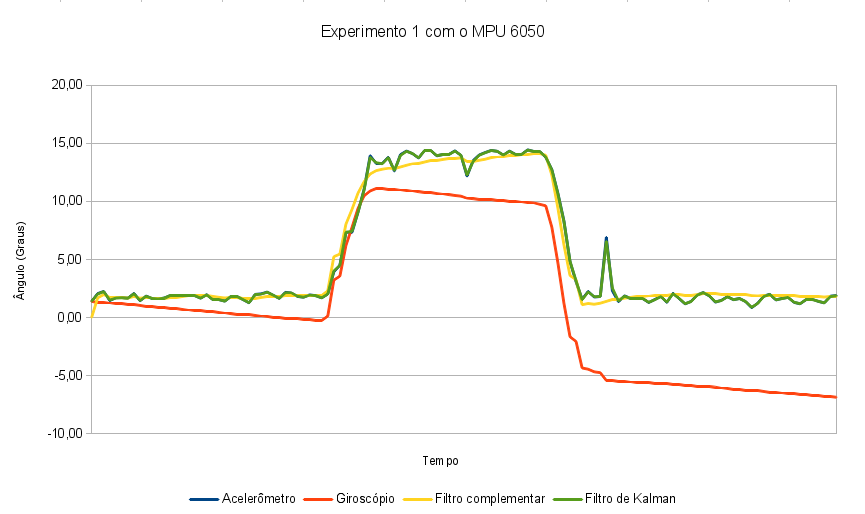
\includegraphics[width=.8\textwidth]{img/exp1.png}
\caption{Primeiro experimento realizado comparando as diferentes formas de medição}
\label{exp1}
\end{figure}

No segundo experimento elevamos o ângulo de forma bastante rápida até cerca de $30^\circ$ e depois o abaixamos, também rapidamente, até próximo de $-5^\circ$. Podemos ver novamente que o filtro complementar é o mais estável e que o filtro de Kalman praticamente acompanha o acelerômetro. Da mesma forma que no outro teste, o giroscópio apresentou o arrasto esperado, variando a media ao longo do tempo, conforme podemos conferir na figura \ref{exp2}. A subida mais íngreme acontece por causa da velocidade mais alta com que o vetor foi girado, sendo que a taxa de variação dessa reta é a velocidade angular nesse período de tempo.

\begin{figure}[H]
\centering
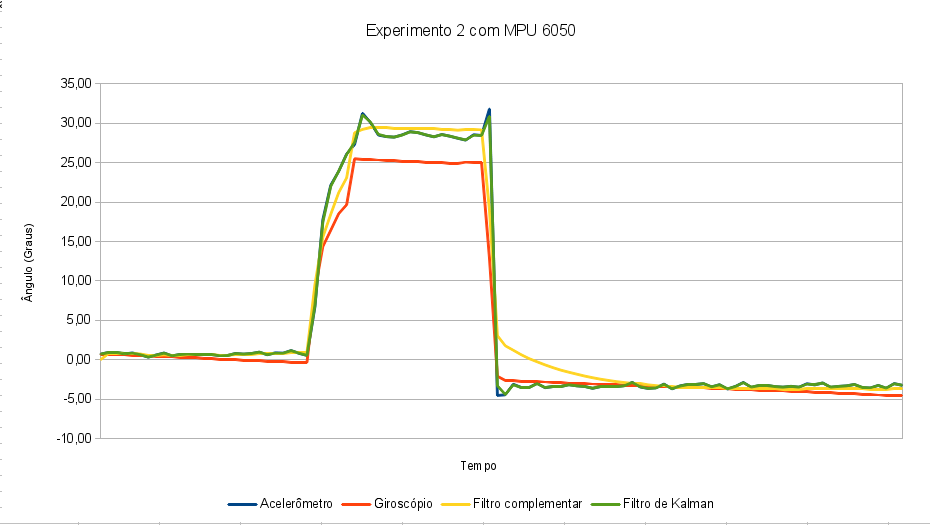
\includegraphics[width=.8\textwidth]{img/exp2.png}
\caption{Segundo experimento realizado comparando as diferentes formas de medição}
\label{exp2}
\end{figure}

No último experimento demonstrativo que fizemos (figura \ref{exp3}), depois da subida e da descida, podemos ver claramente o arrasto ao qual o giroscópio é submetido. Enquanto as outras medidas estavam relativamente estáveis ao longo do tempo o giroscópio foi modificando seu valor ao longo do tempo. Enquanto isso, a medida lida pelo acelerômetro apresenta bastante ruído de alta frequência. Já o filtro complementar se mostra mais estável, sendo capaz de remover grande parte do ruído de alta frequência e eliminando totalmente o ruído de baixa frequência causado pelo giroscópio. 

\begin{figure}[H]
\centering
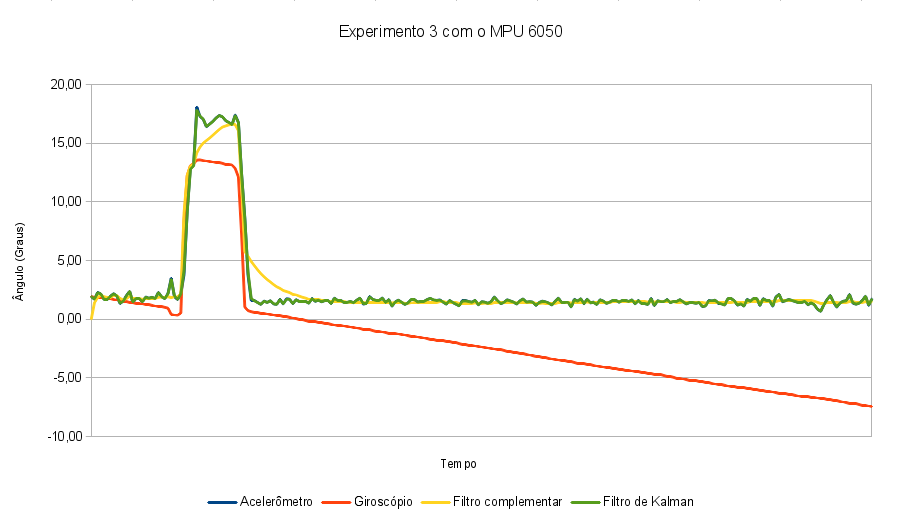
\includegraphics[width=.8\textwidth]{img/exp3.png}
\caption{Terceiro experimento realizado comparando as diferentes formas de medição}
\label{exp3}
\end{figure}

Dos resultados analisados nos gráficos acima apresentados, podemos concluir que, sem uma calibração mais precisa, o filtro de Kalman se mostra ineficiente na remoção do ruído de alta frequência apresentado pelo acelerômetro. Um melhor ajuste em seus parâmetros significa um estudo mais aprofundado do funcionamento do sensor e do comportamento de seus ruídos, sendo necessários extensos testes e estudos estatísticos para tal. Além disso, para uma aferição precisa do sensor, é necessário um inclinômetro externo previamente calibrado. Esse tipo de aparelho, mesmo os portáteis e domésticos, custam centenas de reais, o que nos fez optar por uma medição visual usando um transferidor. Com isso em mente e tendo observado a estabilidade do filtro complementar, podemos concluir que é mais simples e rápido implementar um inclinômetro de baixo custo utilizando esse algoritmo, inclusive pela sua simplicidade e baixo custo computacional.

As medições com o acelerômetro e o giroscópio separados são, como já era esperado, menos precisas do que a combinação das duas, apesar do filtro de Kalman ter praticamente ignorado os dados vindos do giroscópio e acompanhado o sinal do acelerômetro.

Outros fatores também não foram considerados, como a temperatura, que pode interferir nas medições, e vibrações externas, como os motores dos guindastes. A viabilização comercial desse tipo de produto depende primeiramente da consolidação de um projeto de eletrônica que suporte as intempéries das possíveis variações e picos da fonte, a vibração constante dos motores a diesel desses equipamentos, poeira, possíveis respingos e produtos químicos como graxas e óleos. Além disso é necessário se ter uma planejamento de marketing e uma ampla pesquisa de mercado. 

Pensando no possível lançamento de um produto, procuramos por uma empresa de projeto eletrônico e uma de consultoria em guindastes para nos auxiliar no planejamento de tal empreitada. Chegamos a conclusão de que o ideal seria comprarmos os sensores já homologados, aferidos e calibrados por empresas do ramo e montarmos apenas a placa que faria a interface entre os sensores e a máquina. Descobrimos porém que esse mercado já está praticamente saturado, graças à expansão da Vale em Minas Gerais. Como eles exigem que um kit de segurança para qualquer veículo que trafegue em suas minas, surgiu no mercado o chamado ``kit Vale", que consiste em um grupo de sensores como inclinômetro, sensor de comprimento de lança, sensor de pressão de patola entre vários outros. Por essa razão o maior mercado é para kits completos de sensores, que atualizam de uma só vez uma máquina que estava fora dos padrões de segurança.

Entre os sensores exigidos pelas empresas está o de pressão de patola. Esse sensor mede a pressão do fluido hidráulico que sustenta a patola. Com essa medida é possível calcular a carga que está sendo feita sobre aquele ponto e, assim, impedir que o operador do guindaste faça uma operação que o colocará em risco. Esse sensor deve ser instalado no sistema hidráulico do guindaste, que sustenta todo o peso do equipamento sobre as patolas. Caso haja um rompimento desse sistema a máquina provavelmente tombará, causando um acidente potencialmente fatal. A instalação desse sensor é, portanto, crítica e pode afetar o funcionamento do guindaste. Por isso poucos profissionais se arriscam a fazer esse tipo de instalação e, os que tem gabarito para tal, cobram o preço do risco que assumem.

Considerando os fatores de mercado, que exigiriam que expandíssemos o nosso plantel de sensores, as questões técnicas, pelo fato de necessitarmos de mão de obra extremamente especialisada e ainda por não termos garantia de um retorno, optamos por não comercializar o projeto, ficando então a experiência registrada para que possa ser replicada.

\section{Anexos}
\label{anexos}

\subsection{Código desenvolvido}
{\singlespace\begin{lstlisting}
/* Codigo criado originalmente por Kristian Lauszus e modificado para este
   projeto por Gabriel Fonseca sobre os termos da licenca GPL2.
 
 This software may be distributed and modified under the terms of the GNU
 General Public License version 2 (GPL2) as published by the Free Software
 Foundation and appearing in the file GPL2.TXT included in the packaging of
 this file. Please note that GPL2 Section 2[b] requires that all works based
 on this software must also be made publicly available under the terms of
 the GPL2 ("Copyleft").
 
 Informacoes para contato
 -------------------
 
 Kristian Lauszus, TKJ Electronics
 Web      :  http://www.tkjelectronics.com
 e-mail   :  kristianl@tkjelectronics.com
 
 Gabriel Fonseca
 e-mail   :  gabrielmcf@gmail.com
 */

//Controla a comunicacao com o sensor
#include <Wire.h>

//Implementacao do filtro de Kalman para calculo de angulo
// Source: https://github.com/TKJElectronics/KalmanFilter
#include "Kalman.h" 

//Controla o visor LCD
#include <LCD5110_Basic.h>

//Controla a gravacao da calibragem do sensor
#include <EEPROMEx.h>

/**** Pinos do visor ****/
// digital 8  - SCE
// digital 9  - RST
// digital 10 - D/C
// digital 11 - DN (MOSI)
// digital 12 - SCLK
// 5v         - VDD
// digital 6 - led

// Pinos do sensor
// analog 4   - SDA
// analog 5   - SCL
// 3.3v       - VDD

// Botoes
// digital 7 - botao led visor
// digital 4 - botao calibragem

/*********  Declaracao das Variaveis  ***********/

//Variaveis do angulo
Kalman kalmanX; // Create the Kalman instances
Kalman kalmanY;

int16_t accX, accY, accZ;
int16_t gyroX, gyroY, gyroZ;

// Angle calculate using the accelerometer
double accXangle, accYangle; 
// Angle calculate using the gyro
double gyroXangle, gyroYangle; 
// Calculate the angle using a complementary filter
double compAngleX, compAngleY;
// Calculate the angle using a Kalman filter 
double kalAngleX, kalAngleY; 

uint32_t timer;
uint8_t i2cData[14]; // Buffer for I2C data

// Variaveis para o LED
const int pinoBotaoLed = 7;
const int pinoLed = 6;

int statusLed = LOW;
int statusBotaoLed;
int ultimoStatusBotaoLed = LOW;
int leituraBotaoLed;

long ultimoTempo = 0;
long delayTempo = 10;

// Variaveis para a calibracao

const int pinoCalibr = 4;

//ms. Quanto tempo ate ativar o botao
long tempoAtivacao = 5000; 

int ultimoStatusBotaoCalibr = LOW;
int leituraBotaoCalibr;

long tempoPressionado;
long tempoLiberado;

boolean ignorar = false;

//Variaveis do visor
LCD5110 myGLCD(12,11,10,9,8);
extern uint8_t SmallFont[];

double calibragem = 0;

/* Funcoes do sistema */


void calibra(){

  leituraBotaoCalibr = digitalRead(pinoCalibr);

  // Botao pressionado, comeca a contagem
  if (leituraBotaoCalibr == HIGH && 
      ultimoStatusBotaoCalibr == LOW){
    tempoPressionado = millis();
  }
  
  // Botao pressionado por tempo maior que o configurado
  if (leituraBotaoCalibr == HIGH && 
      ultimoStatusBotaoCalibr == HIGH && 
      (millis() - tempoPressionado) > tempoAtivacao){
    myGLCD.clrScr();
    myGLCD.print("CALIBRAGEM", CENTER, 0);
    myGLCD.print("Nivele o ", LEFT, 16);
    myGLCD.print("equipamento.", LEFT, 24);
    myGLCD.print("Aperte o botao", LEFT, 32);
    myGLCD.print("uma vez.", LEFT, 40);

    delay(2000);

    leituraBotaoCalibr = digitalRead(pinoCalibr);

    while(leituraBotaoCalibr != HIGH){
      leituraBotaoCalibr = digitalRead(pinoCalibr);
      ultimoStatusBotaoCalibr = leituraBotaoCalibr;
      
      if(digitalRead(pinoBotaoLed) == HIGH){
        calibragem = 0;
        EEPROM.updateDouble(0,calibragem);
        myGLCD.clrScr();
        myGLCD.print("CALIBRAGEM 0", CENTER, 16);
        delay(3000);
        return;
      }
    }
    
    myGLCD.clrScr();
    myGLCD.print("CALIBRANDO", CENTER, 16);
    
    double valor = kalAngleX;
    
    for (int i = 0; i < 10; i++){
      
      atualizaValores();
      
      valor += kalAngleX;
      valor = valor/2;
      
      delay(200);
    }
    
    calibragem = valor;
    EEPROM.updateDouble(0,calibragem);

    myGLCD.clrScr();    
    myGLCD.print("PRONTO!", CENTER, 0);
    myGLCD.print("Equipamento", CENTER, 24);
    myGLCD.print("calibrado!", CENTER, 32);
    delay(3000);
  }
  
  ultimoStatusBotaoCalibr = leituraBotaoCalibr;

}

// Imprime no visor e no terminal serial
void escreveDados(int exibe){
  
  myGLCD.clrScr();
  myGLCD.print("Angulos", CENTER, 0);
  myGLCD.print("X", 25, 8);
  myGLCD.print("Y", 72, 8);
  myGLCD.print("Ac:", LEFT, 16);
  myGLCD.printNumF(accXangle-calibragem, 1, 20, 16);
  myGLCD.printNumF(accYangle, 1, RIGHT, 16);
  myGLCD.print("Gi:", LEFT, 24);
  myGLCD.printNumF(gyroXangle-calibragem, 1, 20, 24);
  myGLCD.printNumF(gyroYangle, 1, RIGHT, 24);
  myGLCD.print("Co:", LEFT, 32);
  myGLCD.printNumF(compAngleX-calibragem, 1, 20, 32);
  myGLCD.printNumF(compAngleY, 1, RIGHT, 32);
  myGLCD.print("Ka:", LEFT, 40);
  myGLCD.printNumF(kalAngleX-calibragem, 1, 20, 40);
  myGLCD.printNumF(kalAngleX, 1, RIGHT, 40);

  
  if(exibe == 1){  
    Serial.print(accXangle);
    Serial.print("\t");
    Serial.print(gyroXangle);
    Serial.print("\t");
    Serial.print(kalAngleX);
    Serial.print("\t");
    Serial.println(compAngleX);
  }
  
  delay(100);  
}

// Liga e desliga a luz de fundo do visor
void ligaLuz(){
   leituraBotaoLed = digitalRead(pinoBotaoLed);
  
  //Botao pressionado, aciona timer
  if (leituraBotaoLed != ultimoStatusBotaoLed) {
    ultimoTempo = millis();
  }
  
  if((millis() - ultimoTempo) > delayTempo){
    if (leituraBotaoLed != statusBotaoLed){
      statusBotaoLed = leituraBotaoLed;
      
      if (statusBotaoLed == HIGH){
        statusLed = !statusLed;
      }
    }
  }
  
  digitalWrite(pinoLed, statusLed);
  
  ultimoStatusBotaoLed = leituraBotaoLed;
  
}

// Le os valores dos sensores e calcula os angulos
void atualizaValores(){
  while(i2cRead(0x3B,i2cData,14));
  accX = ((i2cData[0] << 8) | i2cData[1]);
  accY = ((i2cData[2] << 8) | i2cData[3]);
  accZ = ((i2cData[4] << 8) | i2cData[5]);
  gyroX = ((i2cData[8] << 8) | i2cData[9]);
  gyroY = ((i2cData[10] << 8) | i2cData[11]);
  gyroZ = ((i2cData[12] << 8) | i2cData[13]);
  
  accXangle = (atan2(accY,accZ))*RAD_TO_DEG;
  accYangle = (atan2(accX,accZ))*RAD_TO_DEG;
  
  //Calculo do angulo usando o giroscopio
  double gyroXrate = (double)gyroX/131.0;
  double gyroYrate = (double)gyroY/131.0;
  
  // Calculo sem filtros  
  gyroXangle += gyroXrate*((double)(micros()-timer)/1000000); 
  gyroYangle += gyroYrate*((double)(micros()-timer)/1000000);
  
  //Calculo usando o filtro complementar
  compAngleX = (0.06*
               (compAngleX+(gyroXrate*(double)(micros()-timer)/1000000)))+
               (0.94*accXangle);
  compAngleY = (0.06*
               (compAngleY+(gyroYrate*(double)(micros()-timer)/1000000)))+
               (0.94*accYangle);
  
  //Calculo usando o filtro de Kalman
  kalAngleX = kalmanX.getAngle(
              accXangle, gyroXrate, (double)(micros()-timer)/1000000);
  kalAngleY = kalmanY.getAngle(
              accYangle, gyroYrate, (double)(micros()-timer)/1000000);
  
}

/************  Configuracao do sistema  ******************/
void setup() {  
  
  //Inicializa comunicacao serial com o computador
  Serial.begin(115200);
  
  //Inicializa o visor LCD
  myGLCD.InitLCD();
  myGLCD.setFont(SmallFont);
  
  myGLCD.print("Iniciando...", LEFT, 0);
  
  Wire.begin();
  
  i2cData[0] = 7; // Set the sample rate
  i2cData[1] = 0x00; // Set Gyro and Acc filtering and sampling
  i2cData[2] = 0x00; // Set Gyro Full Scale Range to +-250deg/s
  i2cData[3] = 0x00; // Set Accelerometer Full Scale Range to +-2g
  while(i2cWrite(0x19,i2cData,4,false)); // Write to registers
  while(i2cWrite(0x6B,0x01,true)); // Disable sleep mode 
  
  while(i2cRead(0x75,i2cData,1));
  if(i2cData[0] != 0x68) { // Read "WHO_AM_I" register
    myGLCD.print("ERRO NO SENSOR!", LEFT, 8);
    //Serial.print(F("Error reading sensor"));
    while(1);  
  }
  
  delay(100); // Wait for sensor to stabilize
  
  myGLCD.print("Sen. config.", LEFT, 8);
  
  /* Set kalman and gyro starting angle */
  while(i2cRead(0x3B,i2cData,6));
  accX = ((i2cData[0] << 8) | i2cData[1]);
  accY = ((i2cData[2] << 8) | i2cData[3]);
  accZ = ((i2cData[4] << 8) | i2cData[5]);
  // atan2 outputs the value of -Pi to Pi (radians)
  // see http://en.wikipedia.org/wiki/Atan2
  // We then convert it to 0 to 2Pi and then from radians to degrees
  accYangle = atan2(accX,accZ)*RAD_TO_DEG;
  accXangle = atan2(accY,accZ)*RAD_TO_DEG;
  
  kalmanX.setAngle(0); // Set starting angle
  kalmanY.setAngle(0);
  gyroXangle = accXangle;
  gyroYangle = accYangle;
  compAngleX = accXangle;
  compAngleY = accYangle;
    
    
  myGLCD.print("Sen. calibr.", LEFT, 16);  


  // Calibragem dos fatores do filtro de Kalman
  
  kalmanX.setQangle(0.01);
  kalmanX.setQbias(0.0003);
  kalmanX.setRmeasure(0.15);

  kalmanY.setQangle(0.01);
  kalmanY.setQbias(0.0003);
  kalmanY.setRmeasure(0.15);
  
  myGLCD.print("Filtro calibr.", LEFT, 24);

  // Calibragem do angulo inicial
  calibragem = EEPROM.readDouble(0);
  
  
  // Luz do visor
  pinMode(pinoBotaoLed, INPUT);
  pinMode(pinoLed, OUTPUT);
  
  digitalWrite(pinoLed, statusLed);
  
  // Botao de Calibragem
  
  pinMode(pinoCalibr, INPUT);
  
  myGLCD.print("PRONTO!", LEFT, 32);
  delay(3000);
  
  timer = micros();
}


/*********   Loop do sistema *********/
void loop() {
  
  // Sub-rotina de calibragem
  calibra();
  
  // Luz do visor
  ligaLuz();

  escreveDados(1);
  
  // Atualiza valores  
  atualizaValores();
  
  // Atualiza contador  
  timer = micros();  
}
\end{lstlisting}
}
\subsection{Biblioteca de filtro de Kalman}

{\singlespace\begin{lstlisting}
/* Copyright (C) 2012 Kristian Lauszus, TKJ Electronics. All rights reserved.
 
 This software may be distributed and modified under the terms of the GNU
 General Public License version 2 (GPL2) as published by the Free Software
 Foundation and appearing in the file GPL2.TXT included in the packaging of
 this file. Please note that GPL2 Section 2[b] requires that all works based
 on this software must also be made publicly available under the terms of
 the GPL2 ("Copyleft").
 
 Contact information
 -------------------
 
 Kristian Lauszus, TKJ Electronics
 Web      :  http://www.tkjelectronics.com
 e-mail   :  kristianl@tkjelectronics.com
 */

#ifndef _Kalman_h
#define _Kalman_h

class Kalman {
public:
    Kalman() {
        /* We will set the varibles like so, these 
           can also be tuned by the user */
        
        Q_angle = 0.001;
        Q_bias = 0.003;
        R_measure = 0.03;
        
        bias = 0; // Reset bias
        P[0][0] = 0.7; // Since we assume tha the bias 
                       // is 0 and we know the starting 
                       // angle (use setAngle), the error 
                       // covariance matrix is set like so - see:
                       // http://en.wikipedia.org/wiki/Kalman_filter
        P[0][1] = 0;
        P[1][0] = 0;
        P[1][1] = 0.7;
    };
    // The angle should be in degrees and the rate should be 
    //in degrees per second and the delta time in seconds
    double getAngle(double newAngle, double newRate, double dt) {
        // KasBot V2  -  Kalman filter module - 
        // http://www.x-firm.com/?page_id=145
        // Modified by Kristian Lauszus
        // See my blog post for more information: 
        // http://blog.tkjelectronics.dk
                        
        // Discrete Kalman filter time update 
        // equations - Time Update ("Predict")
        // Update xhat - Project the state ahead
        /* Step 1 */
        rate = newRate - bias;
        angle += dt * rate;
        
        // Update estimation error covariance - 
        // Project the error covariance ahead
        /* Step 2 */
        P[0][0] += dt * (dt*P[1][1] - P[0][1] - P[1][0] + Q_angle);
        P[0][1] -= dt * P[1][1];
        P[1][0] -= dt * P[1][1];
        P[1][1] += Q_bias * dt;
        
        // Discrete Kalman filter measurement 
        // update equations - Measurement Update ("Correct")
        // Calculate Kalman gain - Compute the Kalman gain
        /* Step 4 */
        S = P[0][0] + R_measure;
        /* Step 5 */
        K[0] = P[0][0] / S;
        K[1] = P[1][0] / S;
        
        // Calculate angle and bias - Update estimate 
        // with measurement zk (newAngle)
        /* Step 3 */
        y = newAngle - angle;
        /* Step 6 */
        angle += K[0] * y;
        bias += K[1] * y;
        
        // Calculate estimation error covariance - 
        // Update the error covariance
        /* Step 7 */
        P[0][0] -= K[0] * P[0][0];
        P[0][1] -= K[0] * P[0][1];
        P[1][0] -= K[1] * P[0][0];
        P[1][1] -= K[1] * P[0][1];
        
        return angle;
    };
    
    // Used to set angle, this should be set as the starting angle
    void setAngle(double newAngle) { angle = newAngle; }; 
    double getRate() { return rate; }; // Return the unbiased rate
    
    /* These are used to tune the Kalman filter */
    void setQangle(double newQ_angle) { Q_angle = newQ_angle; };
    void setQbias(double newQ_bias) { Q_bias = newQ_bias; };
    void setRmeasure(double newR_measure) { R_measure = newR_measure; };
    
private:
    /* Kalman filter variables */
    // Process noise variance for the accelerometer
    double Q_angle;
    // Process noise variance for the gyro bias 
    double Q_bias; 
    // Measurement noise variance - this is actually 
    // the variance of the measurement noise
    double R_measure; 
    
    // The angle calculated by the Kalman 
    // filter - part of the 2x1 state matrix
    double angle;
    // The gyro bias calculated by the Kalman 
    // filter - part of the 2x1 state matrix 
    double bias; 
    // Unbiased rate calculated from the rate 
    // and the calculated bias - you have to call 
    // getAngle to update the rate
    double rate; 
    
    // Error covariance matrix - This is a 2x2 matrix
    double P[2][2];
    // Kalman gain - This is a 2x1 matrix 
    double K[2];
    // Angle difference - 1x1 matrix 
    double y; 
    // Estimate error - 1x1 matrix
    double S; 
};

#endif
\end{lstlisting}}

\section{Bibliografia}

\begin{enumerate}
\item \textsc{Guide to gyro and accelerometer with Arduino including Kalman filtering.} Disponível em: \href{http://www.instructables.com/id/Guide-to-gyro-and-accelerometer-with-Arduino-inclu}{$<$http://www.instructables.com/id/Guide-to-gyro-and-accelerometer-with-Arduino-inclu/$>$}. Acesso em: 25 de mar. 2014.

\item \textsc{A practical approach to Kalman filter and how to implement it.} Disponível em: \href{http://blog.tkjelectronics.dk/2012/09/a-practical-approach-to-kalman-filter-and-how-to-implement-it/}{$<$http://blog.tkjelectronics.dk/2012/09/a-practical-approach-to-kalman-filter-and-how-to-implement-it/$>$}. Acesso em 25 de mar. 2014.

\item \textsc{Higgins jr.}, W. T. A Comparison of Complementary and Kalman Filtering. \textit{IEEE Transactions on Aerospace and Electronic Systems} Vol. AES-11, No. 3, p. 321-325, 1975.

\end{enumerate}

\end{document}
